
\documentclass{article} %
\usepackage{iclr2027_conference,times}

\usepackage[dvipsnames, table]{xcolor}

\usepackage{mathtools}
\usepackage{amsmath}
\usepackage{amssymb}
\usepackage{amsthm}

\usepackage{graphicx}
\graphicspath{{./}{figures/}}
\usepackage[labelformat=simple]{subcaption}
\renewcommand\thesubfigure{(\alph{subfigure})}
\renewcommand\thesubtable{(\alph{subtable})}
\newcommand{\indep}{\rotatebox[origin=c]{90}{$\models$}}
\usepackage{booktabs}
\usepackage{multirow}
\usepackage{tabularx}
\usepackage{placeins}

\usepackage{enumitem}

\usepackage{algorithm}
\usepackage{algorithmic}
\renewcommand{\thealgorithm}{\arabic{algorithm}}

\usepackage{tikz}
\usetikzlibrary{positioning}

\usepackage{listings}
\lstset{
  basicstyle=\small\ttfamily,
  breaklines,
}

\usepackage{microtype}

\usepackage{xspace}
\makeatletter
\def\@onedot{\ifx\@let@token.\else.\null\fi\xspace}
\def\onedot{\futurelet\@let@token\@onedot}
\def\eg{e.g\onedot} \def\Eg{E.g\onedot}
\def\ie{i.e\onedot} \def\Ie{I.e\onedot}
\def\cf{cf\onedot} \def\Cf{Cf\onedot}
\def\etc{etc\onedot} \def\vs{vs\onedot}
\def\iid{i.i.d\onedot} \def\wolog{w.l.o.g\onedot}
\def\wrt{w.r.t\onedot} \def\etal{et al\onedot}
\makeatother

\usepackage{hyperref}
\usepackage{url}
\hypersetup{
  colorlinks,
  linkcolor = BrickRed,
  citecolor = NavyBlue,
  urlcolor  = Magenta!80!black,
}

\theoremstyle{plain}
\newtheorem{theorem}{Theorem}[section]
\newtheorem{proposition}[theorem]{Proposition}
\newtheorem{lemma}[theorem]{Lemma}
\newtheorem{corollary}[theorem]{Corollary}
\theoremstyle{definition}
\newtheorem{definition}[theorem]{Definition}
\newtheorem{assumption}[theorem]{Assumption}
\theoremstyle{remark}
\newtheorem{remark}[theorem]{Remark}

\newcommand{\cmark}{\checkmark}
\newcommand{\xmark}{\times}

\newcommand{\fitwidth}[1]{%
  \resizebox{\ifdim\width>\linewidth\linewidth\else\width\fi}{!}{#1}}

\newcommand{\figureorplaceholder}[2]{%
  \IfFileExists{#1}{\includegraphics[width=\linewidth]{#1}}{%
    \fbox{\parbox[b][0.28\linewidth][c]{0.95\linewidth}{\centering\small
      \texttt{\detokenize{#1}} not found in this checkout.\\[2pt] #2}}}%
}

\title{Do Large Language Models Learn Order-Dependent Rules?}
\author{Anonymous authors \\
Paper under double-blind review}

\begin{document}
\maketitle

\begin{abstract}
Can large language models (LLMs) capture sequential structure when outcomes depend on order? We study this in a controlled, semantic-free sequence framework with three mechanisms over a hidden set of key letters: ordered compliance, driven by key order at a fixed lag; global-property compliance, driven by the parity of the total key count; and key-inversion parity, driven by the parity of key-order inversions. Theoretically, we prove that ordered-compliance inherently leaks information through frequency patterns, creating predictive shortcuts that allow models to succeed without truly capturing causal sequential structure. To isolate true order learning, we introduce a shortcut-auditing protocol that quantifies the predictive power of non-sequential features (e.g., $k$-grams, pair counts) under label noise. Empirically, encoder and recurrent models reach the theoretical optimum (measured by AUC and F1) on ordered-compliance more efficiently than fine-tuned decoder-only LLMs. On global-property compliance, the tested sequence models remain near chance under standard training unless explicitly guided on feature relevance. On key-inversion parity, recurrent and transformer models can solve the task with four keys, while all tested models remain near chance with six. Our results demonstrate that high quality performance on order-sensitive tasks often masks shortcut exploitation, highlighting the need to test whether simpler statistical patterns can explain comparable predictive performance.
\end{abstract}

\section{Introduction}
\label{sec:introduction}

Consider a clinician reviewing a patient's medical history to predict disease progression. The order of events matters: for predicting \textit{myocardial infarction}, \textit{diabetes mellitus} followed by \textit{visual disturbance} tells a different story than the same two events in reverse order~\citep{edelman2026order_specific_ehr}. 
A patient who experiences the transition from cancer stage 2 to cancer stage 3 is worsening, while the opposite order would indicate an improvement. 
Recent studies of electronic health records (EHR) produce comparator cohorts that keep the same events but change their temporal order, and find that sequence-based disease representations consistently outperform bag-of-events models because the order of disease progression carries prognostic information~\citep{edelman2026order_specific_ehr,beaney2024coded_disease_representations,placido2023pancreatic_trajectories,pollington2026trajectory_review}. Similarly, in recommendation systems, the same items can reflect different user preferences depending on the order in which they were selected~\citep{kimLostSequenceLarge2025b}. In these settings, predictions depend not only on \emph{which} events occurred but also on the \emph{order} in which they occurred. Yet, if a sequential model outperforms a bag-of-events model on order-dependent processes, this does not necessarily mean that it has learned the causal power of the order~\citep{geirhos2020shortcut,mccoy2019right}. Sequential data contain many overlapping signals: which events occur, how often, when, and which tend to appear together. A model can use any of these statistics to predict the outcome, if useful, without ever recovering the order-based rule that actually generates the outcome. We call any such signal a \emph{predictive shortcut}: a set of statistics computed from the input sequence that permits above-chance prediction of the label without being sufficient to recover the intended label-generating mechanism. The difficulty is that real-world event trajectories rarely come with a known underlying mechanism, and the space of possible shortcuts is open-ended. LLMs and other transformer-based sequential models are increasingly used for clinical event prediction, sequential recommendation, and temporal reasoning~\citep{savcisens2024using,delphi2025transformer,li2020behrt,rasmy2021medbert,fatemiTESTTIMEBENCHMARK2025}. We therefore focus on evaluating LLMs and other transformer-based models on sequential tasks and comparing their performance against recurrent neural networks, gradient-boosted trees such as XGBoost, and other statistical baselines.

In general, does the performance of LLMs on sequential data reveals anything about how and whether the LLM learns the output-generating mechanism? Recent evidence suggests it may not: LLM-based recommenders often retain most of their performance even when the item order is shuffled~\citep{kimLostSequenceLarge2025b}, and transformer predictions can often be approximated by simple $k$-gram statistics\footnote{$k$-gram statistics are the frequency distributions of contiguous sequences of length k (characters, words, or tokens) extracted from text. Unigrams (k = 1), bigrams (k = 2), trigrams (k = 3), etc., capture local sequential patterns and are fundamental in many NLP applications~\citep{kgram}.}~\citep{nguyen2024understanding}. This motivates us to design a controlled framework based on sequences of letters that deliberately removes meaning and world knowledge. We introduce \emph{ordered-compliance} (OC): a semantic-free abstraction in which a hidden subset of letters (keys) must satisfy a secret ordering rule at a fixed lag to produce a favorable outcome. While label prediction is genuinely order-sensitive, predictive shortcuts may remain available. Therefore, high performance on OC tasks alone cannot distinguish capturing of the intended rule from exploitation of a shortcut.

To complement OC, we introduce two further classes of tests, \emph{key-inversion-parity} (KIP) and \emph{global-property-compliance} (GPC) as stress-test controls. All three classes of tasks share two ingredients: only a hidden subset of letters is relevant, and labels depend on their hidden structure. They progress from an ordering rule which can be substituted with specific shortcuts (OC) to a counting rule that, with balanced sampling, removes predictive shortcuts completely (GPC). KIP is intermediate: order matters, but the label depends on whether the number of key pairs violating the order is even or odd. Neither letter counts nor small subsets reveal the label. GPC removes order dependence by counting key-letter occurrences and assigning label 1 if an even number of key letters have even counts, otherwise 0. In order to justify theoretically our three clases of tasks, under the assumptions in Section~\ref{sec:formulation}, we prove that the three tasks form a progression in how much order matters and how many shortcuts remain. OC uses an explicit order rule, but allows local shortcuts: even a single position carries information about the label, though not necessarily enough to determine it (Theorem~\ref{thm:impossibility}). KIP still depends on order, but only through the number of order violations, and it removes several shortcuts: neither letter counts nor any fixed set of at most $m-2$ positions carries information about the label, where $m$ is the number of key letters (Theorem~\ref{thm:kip_local_purity}). GPC completely eliminates the order and eliminates all local shortcuts: anything shorter than the full sequence provides no information about the label (Theorem~\ref{thm:parity_local_purity}).

We compare LLMs, encoder-only transformers, and recurrent networks across model sizes and training strategies. Using OC, KIP, and GPC, we assess whether these models outperform simpler predictors and baselines that rely just on simple statistics that express predictive shortcuts. We examine both predictive performance and data efficiency, tracking how performance varies with model size and training data quantity. Our comparisons use standard training on the input sequences, without revealing the hidden key letters or providing additional information about the underlying rule. Several models perform well on OC, where however simple statistical baselines can match the best neural models. Success is less consistent on KIP: some models solve the four-key task, but all tested models remain near chance with six keys. On GPC, all the tested models remain near chance. Additional experiments show that providing additional task-relevant information can enable models to solve otherwise unsuccessful KIP and GPC settings. Finally, we apply our approach to a real-world clinical case.

Our findings suggest that the tested models fail to recognize order-dependence as the cause of an outcome, relying instead on predictive shortcuts to achieve high performance. Future theoretical and experimental work is required to verify this hypothesis further.

\paragraph{Contributions.}
\begin{itemize}[leftmargin=*,itemsep=1pt,topsep=2pt]
    \item \textbf{Theory.} We define three label-generating mechanisms over letter sequences (OC, KIP, and GPC) and establish their theoretical properties concerning order dependence and the availability of predictive shortcuts.
    \item \textbf{Shortcut-auditing protocol.} We measure how the predictive performance can be explained by different kinds of shortcuts. We also test how changing event order affects predictions and compare model performance with the theoretical optimum under label noise.
    \item \textbf{Empirical evaluation.} We compare LLMs, encoder-only transformers, and recurrent models across model sizes, training strategies, and training data budgets. We also apply the audits to a real clinical case to assess how much performance can be explained by simpler statistical patterns in real-world sequential tasks.
\end{itemize}

\section{Related work}
\label{sec:related_work}
A growing body of work in domains such as healthcare and recommendation systems suggests that temporal order can add predictive value beyond unordered event identity \citep{beaney2024coded_disease_representations,placido2023pancreatic_trajectories,pollington2026trajectory_review,kimLostSequenceLarge2025b}, and transformer-based models are now routinely applied to longitudinal event histories \citep{li2020behrt,rasmy2021medbert,savcisens2024using,delphi2025transformer}. Of particular relevance, \citet{edelman2026order_specific_ehr} study interpretable \(A\to B\to C\) clinical trajectories using comparator cohorts that preserve event content while changing temporal structure, including \(B\) without prior \(A\), reverse-order, and unordered comparisons. Such settings, together with event-log domains such as predictive process monitoring and system-log anomaly detection \citep{teinemaa2019outcome,du2017deeplog}, motivate our question but cannot answer it directly: sequence-model gains may reflect temporal order, event semantics, co-occurrence, recency, or local event-pattern shortcuts rather than global trajectory reasoning.

Several recent benchmarks probe temporal or sequential ability \citep{fatemiTESTTIMEBENCHMARK2025,cui2025timertemporalinstructionmodeling}, but \citet{klenitskiyDoesItLook2024} argue that many datasets marketed as sequential do not in fact require strong sequential modeling. Consistent with this, transformer behavior is often well approximated by local statistics or $k$-gram rules \citep{nguyen2024understanding,kimLostSequenceLarge2025b,bediFidelityMedicalReasoning2025}, connecting to the broader shortcut-learning literature \citep{mccoy2019right,geirhos2020shortcut,mirzadeh2024gsm}. At the same time, sequential models can in principle realize dependencies beyond fixed \(k\)-gram rules \citep{guMambaLinearTimeSequence2024}. Recent work has introduced tunable synthetic benchmarks for reasoning and sequence processing \citep{kaiserCogniLoadSyntheticNatural2025,ramezanaliSeqBenchTunableBenchmark2025}. Our framework differs by stripping away semantics while enabling a theoretical analysis of the local-information structure of each mechanism. OC suffers unavoidable local leakage; KIP still depends on order but in a less direct manner and restricts the available shortcuts. Balanced GPC removes order dependence entirely, and anything less than the full sequence carries no information about the label.

\section{Methods and theory}
\label{sec:formulation}
We study three label-generating \emph{mechanisms}: ordered compliance (OC), global-property compliance (GPC), and key-inversion parity (KIP). We use the term \emph{task} for the combination of a distribution over input sequences, a mechanism that classifies them, and a label-noise probability. The mechanism assigns each sequence a latent binary label, which is then flipped with the label-noise probability to give the observed label.

\subsection{General setup}
\label{sec:setup}
Let $\mathcal{A}$ be a set of symbols of size $\ell\geq2$, let $n\geq2$ be the sequence length, and write $[h]=\{1,\ldots,h\}$. For each task instance, sample a hidden key set $\mathcal{S}\subseteq\mathcal{A}$ uniformly among subsets of size $m$, where $1\leq m\leq\ell$. For OC and KIP, also sample a uniform bijection $\kappa:\mathcal{S}\to[m]$. These parameters remain fixed across all splits; all probabilities condition on their realized values. GPC uses only $\mathcal{S}$.

For OC and GPC, sequences $X=(X_1,\ldots,X_n)$ are generated
from the distribution $P_0$, defined by
\[
X_t \stackrel{\mathrm{iid}}{\sim} \mathrm{Uniform}(\mathcal{A}),
\qquad t=1,\ldots,n.
\]
so each letter is drawn independently and uniformly from the alphabet $\mathcal{A}$. For KIP, sequences are generated from the conditional distribution
$Q_0$ obtained from $P_0$ by conditioning on each key letter occurring exactly once. An explicit sampling procedure is given in
Definition~\ref{def:kip}.

Each sequence is assigned a latent, noise-free binary label
$Y^*=f(X)\in\{0,1\}$, where $f$ is the deterministic labeling
rule of the chosen mechanism,
corresponding to ordered compliance (OC), global-property
compliance (GPC), and key-inversion parity (KIP), defined below.

To allow for label noise, the observed label $Y$ is generated as
\begin{equation}
\label{eq:label_noise}
Y=Y^*\oplus E,
\qquad E\sim\mathrm{Bernoulli}(\pi),
\qquad E\indep X,
\qquad 0\leq\pi<\tfrac12,
\end{equation}
where $\oplus$ denotes addition modulo two: $E=0$ leaves the
latent label unchanged, whereas $E=1$ flips it. Thus, each label
is flipped with probability $\pi$, independently of the sequence
and independently across examples. Setting $\pi=0$ gives
deterministic labels.

Let $P$ denote the joint distribution of $(X,Y^*,Y)$ induced
by the corresponding input distribution, labeling rule, and
noise model. Write $\rho=P(Y^*=1)$ for the latent positive-class
prevalence.

For $x\in\mathcal{A}^n$ and $a\in\mathcal{A}$, define

\begin{equation}
\label{eq:Na}
N_a(x):=\sum_{t=1}^{n}\mathbf{1}\{x_t=a\},
\qquad
C(x):=(N_a(x))_{a\in\mathcal{A}}.
\end{equation}

These denote the symbol counts and their count vector.
For each position $t\in[n]$, define the membership bit
\begin{equation}
\label{eq:Bt}
B_t:=\mathbf{1}\{X_t\in\mathcal{S}\}.    
\end{equation}

\begin{definition}[Order sensitivity]
\label{def:order_sensitivity}
A task with deterministic labeling rule $f$ is
\emph{order-sensitive} if there exist two sequences $x,x'$
in the input support that contain the same number of
occurrences of each symbol, but satisfy
\[
f(x)\neq f(x').
\]
\end{definition}

\label{sec:pure_sequential_def}

\begin{definition}[Local purity]
\label{def:local_purity}
For a fixed $J\subseteq[n]$, let $X_J=(X_j)_{j\in J}$, ordered by index. A task is \emph{$J$-locally pure} under $P$ if $I_P(Y;X_J)=0$, equivalently $P(Y=1\mid X_J=x_J)=P(Y=1)$ for every positive-probability view $x_J$. For $k\in[n]$, it is \emph{$k$-locally pure} if this holds for every $J$ with $1\leq|J|\leq k$. The same definitions apply to $Y^*$.
\end{definition}

Here $I_P$ denotes mutual information\footnote{\[
I_P(Y;X_J)
=
\sum_{y\in\{0,1\}}
\sum_{x_J\in\mathcal A^J}
P(Y=y,X_J=x_J)
\log
\frac{
P(Y=y,X_J=x_J)
}{
P(Y=y)P(X_J=x_J)
}.
\]}. Positions in $J$ need not be adjacent. The set $J$ is fixed in advance and does not depend on the realized sequence.  Local purity forms a hierarchy: $k$-local purity implies $j$-local purity for every $1\leq j\leq k$, with larger $k$ imposing a stronger requirement. We call a task
\emph{maximally locally pure} if it is $(n-1)$-locally pure,
meaning that no fixed proper subset of the sequence positions
provides information about the label. For a non-degenerate
latent label, $0<\rho<1$, and the independent label-noise
model above with $\pi<1/2$, this is the strongest possible
level: the full sequence remains informative about the label.

\subsection{Ordered compliance mechanism}
\begin{definition}[Ordered-Compliance Mechanism]
\label{def:compliance}
Under the setup of Section~\ref{sec:setup}, fix an integer lag $\lambda\in[n-1]$. A \emph{$\lambda$-run of key symbols} in a sequence
$X=(X_1,\ldots,X_n)$ is a tuple of positions
\[
r=(t,t+\lambda,\ldots,t+(q-1)\lambda),
\]
where $t,q$ are positive integers satisfying
$t+(q-1)\lambda\leq n$, and
\[
X_{t+i\lambda}\in\mathcal{S}
\qquad
\text{for every }i=0,\ldots,q-1.
\]
The run is \emph{maximal} if it cannot be extended to the left or to the right
by another key symbol at distance $\lambda$; that is, both of the following conditions hold:
\[
\begin{aligned}
&t-\lambda<1
  \quad\text{or}\quad X_{t-\lambda}\notin\mathcal{S},\\
&t+q\lambda>n
  \quad\text{or}\quad X_{t+q\lambda}\notin\mathcal{S}.
\end{aligned}
\]
A maximal $\lambda$-run $r=(t,t+\lambda,\ldots,t+(q-1)\lambda)$ is
\emph{ordered} if $q\geq 2$ and
\[
\kappa(X_t)
\leq
\kappa(X_{t+\lambda})
\leq
\cdots
\leq
\kappa(X_{t+(q-1)\lambda}).
\]
We say that $X$ is \emph{ordered-compliant} (OC) if it contains at least one ordered
maximal $\lambda$-run.

For this mechanism, the labeling rule is $Y^*=f(X)=\mathbf{1}\{X\text{ is ordered-compliant}\}$.

\end{definition}

Maximality excludes increasing pairs inside longer unordered runs: for ranks $A<B<C$, distractor $d$, and $\lambda=1$, $(d,A,B,C,d)$ is compliant but $(d,A,C,B,d)$ is not. Repeated keys are allowed. 

\begin{theorem}[OC contains single-position label information]
\label{thm:impossibility}
Fix $(\mathcal{S},\kappa)$, an integer $\lambda\geq1$, and $n\geq\lambda+1$. More generally than the uniform setting above, suppose $X$ has independent coordinates with full support on $\mathcal{A}$. Let $P$ denote the joint distribution induced by this input distribution, the OC mechanism in Definition~\ref{def:compliance}, and the noise model in~\eqref{eq:label_noise}. Write $\rho=P(Y^*=1)$. If $0<\rho<1$, there exist $a,b\in\mathcal{A}$ such that
\[
P(Y^*=1\mid X_1=a)\neq P(Y^*=1\mid X_1=b).
\]
Consequently, $I_P(Y^*;X_1)>0$ and $I_P(Y;X_1)>0$.
\end{theorem}

The proof is in Appendix~\ref{appendix:proof_impossibility}. Under the assumptions of the theorem, OC fails every positive level of local purity: it is not \(k\)-locally pure for any \(1\leq k\leq n\), since the singleton \(J=\{1\}\) already contains information about the label. 

The OC mechanism represents outcomes that depend on whether some events satisfy a hidden ordering rule. Theorem~\ref{thm:impossibility} shows that this structure also leaks predictive information through single positions: under the theorem's assumptions, even the first position carries information about the label. A predictor, therefore, can exploit shortcuts without reading the whole sequence and hence without identifying the hidden causal mechanism.

\subsection{Key-inversion parity mechanism}
\label{sec:kip}
We introduce key-inversion parity (KIP), an order-sensitive mechanism that is $(m-2)$-locally pure.

\begin{definition}[Key-inversion parity]
\label{def:kip}
Under the setup of Section~\ref{sec:setup}, take $3\leq m\leq n$ and $m<\ell$. Define $Q_0$ as the probability law on $\mathcal{A}^n$ generated by the following procedure: choose $m$ key positions uniformly from the $m$-subsets of $[n]$, assign the keys in $\mathcal{S}$ to those positions by a uniform random bijection, and fill remaining positions independently and uniformly from $\mathcal{A}\setminus\mathcal{S}$, independently of these choices. Each key occurs exactly once. For key positions $T_1<\cdots<T_m$, let $R_i=\kappa(X_{T_i})$, write $R=(R_1,\ldots,R_m)$ and define
\begin{equation}
\label{eq:kip_label}
\operatorname{Inv}(R)=\sum_{1\leq i<j\leq m}\mathbf{1}\{R_i>R_j\},\qquad Y^*=\operatorname{Inv}(R)\bmod2.
\end{equation}
\end{definition}

The exactly-once constraint makes coordinates dependent: KIP differs from OC in both input law and label rule, so the OC theorem does not apply.

\begin{theorem}[Order sensitivity and local purity of KIP]
\label{thm:kip_local_purity}
Under Definition~\ref{def:kip}, let $C(X)=(N_a(X))_{a\in\mathcal{A}}$. Then $P(Y^*=1)=1/2$, and swapping any two keys flips the label while preserving $C(X)$. Moreover,
\[
I_P(Y^*;C(X))=0,\qquad I_P(Y^*;X_J)=0\quad\text{for every }J\subseteq[n]\text{ with }|J|\leq m-2.
\]
KIP is not $(m-1)$-locally pure, so its threshold is exactly $m-2$. Both independence and failure of $(m-1)$-local purity persist for $Y$ under~\eqref{eq:label_noise}.
\end{theorem}

The proof is in Appendix~\ref{appendix:proof_kip_local_purity}. Our $n=20$, $m\in\{4,6\}$, $\pi=0$ settings have exact purity through two and four positions. In KIP, symbol counts alone provide no information about the label.

\subsection{Global-property compliance mechanism}
\label{sec:parity}
We finally introduce global-property compliance (GPC), a mechanism that is not order-sensitive and satisfies $(n-1)$ local purity.

\begin{definition}[Global-property compliance]
\label{def:parity}
Under $P_0$ and the general setup defined of Section~\ref{sec:setup}, take $1\leq m<\ell$. GPC sets $Y^*=1$ when an even number of keys have even counts, including zero occurrences; equivalently,
\begin{equation}
\label{eq:gpc_label}
Y^*=\mathbf{1}\!\left\{\sum_{t=1}^n B_t\equiv m\pmod 2\right\}.
\end{equation}
\end{definition}

To see why the two formulations agree, let \(o\) be the number of keys with odd counts. Then \(m-o\) keys have even counts, and \(\sum_t B_t\equiv o\pmod 2\), since only odd counts contribute to the sum modulo two. Therefore, \(m-o\) is even exactly when \(\sum_t B_t\equiv m\pmod 2\).

\begin{theorem}[Local information in GPC]
\label{thm:parity_local_purity}
Under Definition~\ref{def:parity} and $P_0$, let $p=m/\ell\in(0,1)$. For every nonempty $J\subsetneq[n]$,
\[
I_P(Y^*;X_J)=0\ \text{if }p=\tfrac12,\qquad I_P(Y^*;X_J)>0\ \text{otherwise}.
\]
For fixed $p\neq1/2$ and a fixed finite nonempty index set $J$, this information tends to zero as $n\to\infty$. The same statements hold for $Y$ under~\eqref{eq:label_noise}. Hence balanced GPC ($p=1/2$) is $k$-locally pure for every $1\leq k<n$.
\end{theorem}

The proof is in Appendix~\ref{appendix:proof_parity_local_purity}. 

In essence, our theoretical results serve one purpose: to measure how much a sequential task ishortcut-dominated. OC shows this directly. Its label depends on order, yet even a single position carries information about it, so a model can perform well on OC without using the rule. This motivated KIP and GPC as comparison tests that theoretically allow fewer shortcuts. KIP keeps the label order-dependent and removes two of them: neither letter counts nor any fixed set of at most $m-2$ positions carries information about the label. GPC removes all local shortcuts: anything less than the full sequence carries no information. Comparing a model across the three tasks, and against baselines restricted to the statistics each task allows, is what lets us tell rule learning from shortcut use.

\section{Experiments}
\label{sec:experiments}
We evaluate how well different architectures perform on the tasks built from the three mechanisms defined above and whether they outperform baselines that rely on predictive shortcuts. These tasks vary in whether order matters and in how much information individual positions or small groups of positions provide about the label. We then apply the same evaluation framework to a real-world clinical task in MIMIC-IV~\citep{johnson2023mimiciv}, a widely used database of electronic health records. Code is available in an anonymous repository.

\subsection{Controlled synthetic dataset and task variants}
\label{sec:task_variants}

We instantiate the three mechanisms on sequences of length $n=20$ over an alphabet of $\ell=26$ symbols, yielding five experimental variants.

\textbf{Ordered compliance.}
OC-Deterministic and OC-Noisy use $m=6$ keys and lag $\lambda=7$, with label-noise probabilities $\pi=0$ and $\pi=.3$, respectively. Both have latent positive-class prevalence $\rho\approx .293$. The lag makes the relevant ordering non-adjacent, while the two noise levels allow us to assess the effect of label noise on model performance. Parameter choices and sensitivity analyses are discussed in Appendix~\ref{app:sensitivity}.

\textbf{Key-inversion parity.}
KIP-4 and KIP-6 use four and six keys, respectively, with no label noise and latent positive class prevalence $\rho=.5$. Each key occurs exactly once. By Theorem~\ref{thm:kip_local_purity}, these variants are exactly $2$- and $4$-locally pure, allowing us to compare model performance as both the number of keys and the degree of local purity increase.

\textbf{Global-property compliance.}
GPC-Deterministic uses $m=6$ keys and no label noise, matching the hidden-subset size of the OC variants, with latent positive-class prevalence $\rho\approx .499$. Its label depends on global parity and is invariant to sequence order.

\subsection{Models and baselines}
\label{subsec:models}

We fine-tune pretrained decoder models, Llama-3.2-1B, Llama-3.1-8B, and Llama-3.1-70B~\citep{touvron2023llama,grattafiori2024llama3}, Qwen3-4B-Think~\citep{bai2023qwen}, Qwen2.5-14B~\citep{qwen2.5,qwen2}, and Qwen3.8-27B~\citep{qwen38} and encoder models BERT-base (110M)~\citep{devlin2019bert} and RoBERTa-large (355M)~\citep{liu2019robertarobustlyoptimizedbert} for binary classification. To isolate architecture from pretrained knowledge, we also train randomly initialized Llama-style decoders (1M parameters), LSTMs~\citep{hochreiter1997lstm}, transformer encoders~\citep{vaswani2017attention}, and a hybrid BiLSTM-Transformer~\citep{graves2005bilstm} (called here RNNTransformer). Our baselines include XGBoost~\citep{chen2016xgboost} with integer-encoded letters (XGBoost-basic) or, following~\citet{XGBoost_LLMs,XGBoost_LLMs_HF}, mean-pooled Llama-3.2-1B embeddings (XGBoost-LLM), contiguous $k$-gram scores, and classifiers based on letter counts or ordered pair counts. Pair-count features record how often each ordered pair of letters occurs at a specified distance or across all possible distances. On OC, we compare a baseline given the true lag $\lambda$ with baselines using all $n-1$ possible lags. Regularized logistic regression and boosted trees assess the predictive value of these features. Input encodings and feature definitions are detailed in Appendices~\ref{subsec:encoding}.

\subsection{Training and evaluation}
\label{subsec:training}
\label{subsec:evaluation}

For the controlled synthetic tasks, all neural models are trained for binary classification with early stopping on validation performance with AdamW~\citep{AdamW}. The classification loss is cross-entropy; for causal decoders, the training loss is the sum of cross-entropy loss and a next-token prediction loss computed over the input prompt. We finetuned pretrained models using LoRA~\citep{LoRA} and for big models (27B+ parameters) we use QLoRA~\citep{qlora} with 4-bit precision to reduce memory requirements. The synthetic datasets use an 80/10/10 train/validation/test split. For each task and each model we use 4K, 40K, 120K, 200K, 300K, and 400K training examples in order to check data-efficiency. Experiments run on one NVIDIA H200 GPU (141GB), with three seeds unless otherwise stated. We report test AUC, F1, precision, and recall, using AUC as the primary metric. Model-specific settings are detailed in Appendix~\ref{appendix:training}. We compare performance with the label-noise oracle
(Theorem~\ref{thm:optimal_performance}). $AUC^*$ is the optimal AUC; precision$^*$, recall$^*$, and F1$^*$ refer to the classifier $\hat{Y}=Y^*$. All four values equal $1$ in noise-free settings. For OC-Noisy ($\rho=.293$, $\pi=.3$), the corresponding values are $.670$, $.700$, $.491$, and $.577$, respectively.

\subsection{Real-world case study: chronic kidney disease progression}
\label{subsec:mimic_ckd_protocol}
We focus on predicting progression from chronic kidney disease (CKD) to end-stage renal disease (ESRD) using patient histories. This choice follows previous studies treating the task as sequential prediction~\citep{kip1,kip2,kip3,kip4}. We use MIMIC-IV~\citep{johnson2024mimiciv31,johnson2023mimiciv} and we assess whether the order of recorded diagnoses adds predictive value beyond their identity and frequency. The cohort contains $14\,813$ patients with  CKD, including $1\,146$ positives whose subsequent admissions contain an ESRD-related code. For positive cases, inputs stop before the first ESRD-related admission; patients with CKD and ESRD first recorded in the same admission are excluded. Diagnosis codes are mapped to $293$ Clinical Classifications
Software (CCS) categories~\citep{hcup_ccs}. Admissions are ordered chronologically, while codes within each admission follow administrative billing order. We compare contiguous $k$-gram predictors, bag-of-code baselines, and sequence models using original and shuffled diagnosis histories, with AUC as the main evaluation metric. Details are in Appendix~\ref{appendix:mimic_ckd}.

\section{Results}
\label{sec:results}
\begin{figure}[htbp]
\centering
\includegraphics[width=\linewidth]{auc_main_iclr.png}
\caption{Test AUC versus training-set size on OC-Noisy, KIP-4, and GPC. For readability, we show one representative model per family (full results in Appendix~\ref{appendix:synthetic_results}). Dashed curves labeled \emph{full} denote full fine-tuning; other LLMs use LoRA/QLoRA.}
\label{fig:comparison_AUC_all}
\end{figure}

This section summarizes the main results; the full set, for every model and task, is in Appendices~\ref{appendix:synthetic_results} and~\ref{appendix:mimic_ckd}. Figure~\ref{fig:comparison_AUC_all} shows how test AUC changes with training-set size on the three most informative settings, OC-Noisy, KIP-4, and GPC, for one representative model per family. KIP-6 behaves like GPC, with no model above chance, so its curves are left to the appendix, together with OC-Det.

\paragraph{Ordered compliance.}
On \textbf{OC-Deterministic}, pretrained bidirectional encoders (BERT, RoBERTa) and small randomly initialized sequential models (Transformer, LSTM, RNNTransformer; roughly 80K--220K parameters) reach AUC \(\ge .997\). Decoder-only Llama-3.2-1B plateaus at AUC \(\approx .85\), close to the contiguous 2-gram baseline of 0.82, while Llama-3.1-8B reaches AUC $=.995$. XGBoost on frozen Llama-3.2-1B mean-pooled embeddings also fails; this likely reflects a mismatch between pretrained representations and our synthetic letter task rather than a property of the embedding architecture per se. An $L_2$ logistic regression on the 676-dimensional \(\lambda\)-aware pair feature \(g_{ab}^{(\lambda=7)}\) reaches AUC $=.997$ (Appendix~\ref{appendix:ladder}), and a \(\lambda\)-agnostic $L_1$ logistic regression on the 12\,844-dimensional all-lag stacking recovers \(\lambda=7\) on its own (Appendix~\ref{appendix:lam_agnostic}). We therefore read the encoder--decoder gap on this task as an efficiency gap in discovering the right lagged-pair feature from raw-token supervision, rather than as evidence for global sequence integration. The pair feature is a per-rule weighting rather than a transferable procedure: leave-one-rule-out logistic regression on \(g_{ab}^{(\lambda)}\) reaches within-rule AUC $1.00$ but across-rule AUC $.50$ (Appendix~\ref{appendix:heldout}). On \textbf{OC-Noisy}, BERT, LSTM, the small Transformer, and RNNTransformer reach AUC between $.665$ and $.671$, close to the oracle reference of $.670$. BERT approaches this value with 120K examples. The number of trained parameters also affects performance: Llama-3.2-1B and Llama-3.1-8B reach $.587$ and $.575$ with rank-8 LoRA, but $.670$ and $.668$ with full fine-tuning. BERT reaches $.669$ using LoRA, and Qwen2.5-14B also reaches $.670$ with LoRA. 
When the lag $\lambda$ is given, an $L_2$ logistic regression on $g_{ab}^{(\lambda=7)}$ reaches AUC $=.671$ (Appendix~\ref{appendix:ladder}); without it, XGBoost on pair counts at all lags reaches $.667$. An $L_1$ logistic regression on the same all-lag counts reaches only $.632$: under label noise it fails to identify the features of the correct lag, and its largest weights land on $\lambda=19$ instead of $7$ (Appendix~\ref{appendix:lam_agnostic}).

\paragraph{Key-inversion parity.}
On KIP-4, the LSTM reaches AUC $1.000$ in all three seeds with early-stopping patience 5 (with patience 3, one seed stays at chance; Appendix~\ref{app:kip_controls}). Several pretrained decoders also reach near-perfect AUC: Llama-3.2-1B and Llama-3.1-8B with full fine-tuning, Llama-3.1-8B with LoRA, and Qwen2.5-14B and Qwen3.8-27B with QLoRA. In the data-efficiency sweep, these decoders remain near chance through 120K training examples and reach AUC $1.000$ at 200K (Table~\ref{tab:kip_data_efficiency}). On KIP-6, all tested neural models remain near chance under the same training procedures. Shuffle controls show that successful KIP-4 predictions depend on order (Appendix~\ref{app:kip_controls}). For the LSTM, retraining on shuffled sequences while retaining the original labels yields AUC $.500$, and test-only shuffling of the patience-3 checkpoints yields $.502$. Test-only shuffling also reduces the fully fine-tuned Llama-3.2-1B from $1.000$ to $.505$. For each ordered pair of letters, we count how often the second letter appears $d$ positions after the first, for every distance $d\in\{1,\ldots,n-1\}$, and aggregate these counts over $d$ by their maximum or sum, giving a 676-dimensional feature. XGBoost on this feature reaches AUC $1.000$ on KIP-4 but stays at chance on KIP-6, and logistic regression on it stays at chance on both; keeping the $n-1$ distance-specific counts separate (12\,844 dimensions) gives only $.590$ on KIP-4 (Table~\ref{tab:kip_features}). In a separate experiment, we use the known key set to build an input that says, for each pair of keys, which one occurs first in the sequence. A small MLP trained on this input reaches AUC $1.000$ on both KIP-4 and KIP-6 (Table~\ref{tab:kip_reveal}). Thus, once the keys' relative order is supplied, even KIP-6 is solvable.

\paragraph{Global-property compliance.}
On GPC, all tested models remain near chance (AUC $\approx .50$) in the main $m=6$ regime, including a 70B-parameter LLM, encoder-only transformers, and recurrent networks (Table~\ref{tab:results_full_gpc}). The contiguous $k$-gram baselines remain near chance as well for every $k$ (Appendix~\ref{app:kgram}), consistent with \citet{countingLLMs}. Once key membership is provided, the parity rule becomes learnable (Appendix~\ref{appendix:parity_decomp}). A 64-unit MLP given the membership vector $(B_1,\ldots,B_n)$, where $B_t=\mathbf{1}\{X_t\in\mathcal{S}\}$, reaches AUC $.997$ in under a minute; this $n$-dimensional binary input says which positions hold a key, but not which key. Given the $m$-dimensional per-key parity vector $(N_a(X)\bmod 2)_{a\in\mathcal{S}}$ instead, the same MLP reaches AUC $1.000$ (Table~\ref{tab:parity_decomp}). Results also depend on sequence length: an LSTM (three of three seeds) and a small randomly initialized Transformer (two of three) learn GPC at $n=10$, whereas every model trained directly at $n=20$ remains at chance (Appendix~\ref{app:parity_curriculum}). \citet{hahn-2020-theoretical} identifies length-dependent difficulties for transformer parity learning (the key ingredient of our GPC mechanism), consistent with this observation. We exploit the gap with a two-stage curriculum: train from scratch on $n=10$, then warm-start on $n=20$ with positional embeddings transferred where applicable. This recovers global-property compliance for the LSTM and for the Transformer seeds that solved $n=10$, but not for pretrained BERT under our tested recipe (Appendix~\ref{app:parity_curriculum}).

\paragraph{Chronic kidney disease progression}
For CKD-to-ESRD prediction, unigrams achieve an AUC of $.823$ outperforming contiguous bigrams that reach $.801$ across five patient splits. On a separate split used for bag-of-code and neural models, count-based logistic regression and XGBoost attain AUCs of $.809$ and $.803$, respectively. The Transformer model scores $.860$ with ordered histories and $.844$ when the histories are shuffled; BERT and BiLSTM do not show any positive difference between ordered and shuffled histories. Predictors that only use the presence and frequency of diagnosis codes already achieve about $.810$ AUC. The Transformer performs better with ordered histories, but BERT and BiLSTM show no improvement over the shuffled data. We've realized that there can be significant shortcuts in sequential medical tasks and, as \cite{klenitskiyDoesItLook2024} has pointed out, phenomena that should depend on the temporal ordering of events might be heavily shortcut-dominated, so that good performance on it reveals nothing about whether a model uses order.

\paragraph{Attention diagnostics.}
We inspect attention layer by layer for encoder and decoder-only models on OC, KIP, and the real case study. Notably, among the transformer-based models, only decoder-only models solve KIP-4. Their attention in fact concentrates on key letters, and input perturbations confirm that their predictions are sensitive to key order and stable when distractors are swapped. Results in Appendix~\ref{appendix:attention}.

\section{Discussion and limitations}
\label{sec:limitations}
This work introduces a controlled, semantic-free framework to examine whether a model has learned the underlying causal order-dependent rule whenever its predictive performance is good. Our three frameworks form a progression: from OC, where order takes its simplest form, whether $A$ comes before or after $B$, and for that very reason leaves shortcuts available, to KIP and GPC, where order becomes less and less decisive until it disappears, and fewer or no shortcuts remain available. 

On OC, simple classifiers given lagged-pair counts match the best neural models, so what really matters is how efficiently they discover such features from raw tokens. KIP-4 shows the other side: an LSTM and fine-tuned Llama and Qwen models solve it from raw sequences, where count-based baselines cannot, and the only baseline that matches them is given pair counts aggregated over all lags as input (Appendix~\ref{app:kip_controls}). On KIP-6 and GPC, every model trained on raw sequences stays near chance under standard training, while small MLPs given key membership or the keys' relative order succeed, so the difficulty lies in discovering the hidden structure and learning the rule at the same time. The clinical audit shows why this matters in practice: which diagnoses occur, and how often, already supports strong prediction, and temporal order adds at most a modest gain.

From a theoretical perspective, the OC theorem is specific to the OC mechanism under independent full-support sampling and does not extend to arbitrary order-sensitive labels. The amount of OC label information depends on the sampling distribution. KIP uses dependent inputs and falls outside these assumptions. The local-purity guarantees concern fixed sets of positions and do not exclude informative features computed from the whole sequence. These results describe where label information is available; they do not determine whether a model will learn to use it. Likewise, high AUC and sensitivity to noise do not identify a model’s internal reasoning. Our experimental setting is not a general benchmark for long-range sequential learning. Empirically, we focus on one main regime per task, with sensitivity sweeps and ablations in the appendix; most models are tested up to 27B parameters, with the 70B model evaluated only on the GPC mechanism. The theoretical claims also rely on independent full-support sampling and should not be read as impossibility results for arbitrary real-world sequence distributions, transformers, or parity-like tasks in general.

Finally, we investigated a single clinical case study. However, as recent work highlights \citep{edelman2026order_specific_ehr}, while true temporal dependencies certainly exist in clinical trajectories, they are not trivial to isolate. Therefore, judging a model's architectural adequacy based solely on its performance on real-world sequential tasks requires extreme caution. Nevertheless, our case study efficiently demonstrates a broader fundamental principle: apparent sequentiality in real data does not imply an absence of predictive shortcuts.

\section{AI use statement}
LLMs were used to assist with code debugging and visualization scripts, improve writing, draft selected manuscript sections, and discuss the interpretation and limitations of the results. The authors reviewed and revised the AI-assisted text and take full responsibility for the final content of this work.
\bibliographystyle{iclr2027_conference}
\bibliography{references}

\clearpage
\appendix

\paragraph{Appendix roadmap.}
Proofs: Appendix~\ref{appendix:proof_theorems}; training: Appendix~\ref{appendix:training}; full synthetic results: Appendix~\ref{appendix:synthetic_results}; sensitivity sweep: Appendix~\ref{app:sensitivity}; mechanism-identification audit: Appendix~\ref{appendix:mechanism_id}; clinical audit: Appendix~\ref{appendix:mimic_ckd}; attention diagnostics: Appendix~\ref{appendix:attention}.

\section{Proofs}
\label{appendix:proof_theorems}

All probabilities condition on the realized hidden parameters. The OC theorem
assumes independent coordinates with full support; its quantitative bound uses
the uniform proposal. GPC uses the i.i.d.\ uniform proposal $P_0$, whereas KIP
uses the dependent-input law $Q_0$ of Definition~\ref{def:kip}.
For any statistic $V$ of $X$, independent symmetric label noise gives
\begin{equation}
\label{eq:appendix_noise_channel}
P(Y=1\mid V)=\pi+(1-2\pi)P(Y^*=1\mid V).
\end{equation}
For $\pi<1/2$, this affine map preserves constancy and nonconstancy of the
posterior. We use this observation throughout instead of repeating the
noise calculation in each proof.

\subsection{Oracle performance under label noise}

\begin{theorem}[Oracle AUC and hard-oracle metrics]
\label{thm:optimal_performance}
Suppose $Y^*$ is a deterministic function of $X$, $0<\rho=P(Y^*=1)<1$,
and labels are independently flipped with probability $\pi\in[0,1/2)$.
Set $q=P(Y=1)=\pi+(1-2\pi)\rho$. The Bayes-optimal AUC is
\begin{equation}
\label{eq:oracle_auc_compact}
\mathrm{AUC}^*
=\frac12+\frac12\left(\frac{(1-\pi)\rho}{q}
-\frac{\pi\rho}{1-q}\right)
=\frac12+\frac{\rho(1-\rho)(1-2\pi)}{2q(1-q)}.
\end{equation}
For the hard oracle $\widehat Y=Y^*$, precision, recall, and F1 are
$\mathrm{Prec}_{\rm oracle}=1-\pi$,
$\mathrm{Rec}_{\rm oracle}=(1-\pi)\rho/q$, and
$F_{1,\rm oracle}=2(1-\pi)\rho/[\pi+2(1-\pi)\rho]$.
The latter metrics describe this particular thresholded classifier and are
not asserted to be optimal over thresholds.
\end{theorem}

\begin{proof}
\label{proof:optimal_performance}
The posterior $P(Y=1\mid X)=\pi+(1-2\pi)Y^*$ orders the two latent
classes correctly, so $s=Y^*$ attains Bayes-optimal AUC. Let
$a=P(s=1\mid Y=1)=(1-\pi)\rho/q$ and
$c=P(s=1\mid Y=0)=\pi\rho/(1-q)$. Counting ties with weight $1/2$ gives
\[
\mathrm{AUC}(s)=a(1-c)+\tfrac12\{ac+(1-a)(1-c)\}
=\tfrac12+\tfrac12(a-c).
\]
For the hard oracle, $(\mathrm{TP},\mathrm{FP},\mathrm{FN},\mathrm{TN})
=((1-\pi)\rho,\pi\rho,\pi(1-\rho),(1-\pi)(1-\rho))$;
substitution gives the remaining formulas.
\end{proof}

For $\pi=0$, the oracle metrics equal one; for $\rho=1/2$, they equal $1-\pi$.

\subsection{Proof of Theorem~\ref{thm:impossibility}}
\label{appendix:proof_impossibility}

\begin{proof}
Let $s_{\min}$ and $s_{\max}$ be the lowest- and highest-ranked keys.
We show that $P(Y^*=1\mid X_1=a)$ is nonconstant in $a$.

\textit{Case $\mathcal S\subsetneq\mathcal A$.}
Choose $a_0\notin\mathcal S$ and couple
$\widetilde X=(s_{\min},Z_2,\ldots,Z_n)$ and
$\widetilde X'=(a_0,Z_2,\ldots,Z_n)$, where the $Z_t$ are independent
with the respective laws of $X_t$. Independence makes these the conditional
laws given $X_1=s_{\min}$ and $X_1=a_0$.
Write $C$ and $C'$ for their compliance events. Any ordered maximal
$\lambda$-run in $\widetilde X'$ either remains unchanged in $\widetilde X$
or starts at $1+\lambda$ and extends left by the minimum-ranked key.
The extended run remains ordered and maximal. Thus $C'\subseteq C$.
The event
\[
W=\{Z_{1+\lambda}\in\mathcal S\}
\cap\bigcap_{t\in\{2,\ldots,n\}\setminus\{1+\lambda\}}
\{Z_t\notin\mathcal S\}
\]
has positive probability by full support. On $W$, $\widetilde X$ has the
ordered maximal run $(1,1+\lambda)$, while $\widetilde X'$ has only one
key and is not compliant. Consequently,
\[
P(Y^*=1\mid X_1=s_{\min})-P(Y^*=1\mid X_1=a_0)
=P(C\setminus C')\geq P(W)>.
\]

\textit{Case $\mathcal S=\mathcal A$.}
Maximal runs are the residue classes modulo $\lambda$. Let
$R_1=(1,1+\lambda,\ldots,1+(L-1)\lambda)$,
$L=1+\lfloor(n-1)/\lambda\rfloor\geq2$.
Let $O_1$ denote that $R_1$ is ordered, and $B$ that a different maximal
run is ordered. These events depend on disjoint coordinates, so
\[
P(Y^*=1\mid X_1=a)=P(B)+(1-P(B))P(O_1\mid X_1=a).
\]
Here $P(B)<1$, since otherwise $\rho=1$. Also $|\mathcal A|\geq2$ by
nondegeneracy. Given $X_1=s_{\min}$, $O_1$ requires only that the
remaining entries of $R_1$ be nondecreasing. Given $X_1=s_{\max}$, it
requires that all those entries equal $s_{\max}$. The latter event is
contained in the former; containment is strict with positive probability
because all remaining entries can instead equal $s_{\min}$.
Thus the two compliance posteriors differ.

In both cases, $Y^*$ and $X_1$ are dependent, hence $I(Y^*;X_1)>0$.
Equation~\eqref{eq:appendix_noise_channel} gives $I(Y;X_1)>0$ as well.
\end{proof}

\paragraph{Quantitative bound and sampling scope.}
\label{sec:uniform_witness_bound}
\label{appendix:proof_uniform_witness_bound}

\begin{corollary}[Uniform witness lower bound]
\label{cor:uniform_witness_bound}
Under the OC theorem with $\mathcal S\subsetneq\mathcal A$ and i.i.d.\
uniform inputs, let $m=|\mathcal S|$, $\ell=|\mathcal A|$, and
$\delta(a,b)=P(Y^*=1\mid X_1=a)-P(Y^*=1\mid X_1=b)$. Then
\begin{equation}
\label{eq:witness_clean}
\delta(s_{\min},a_0)\geq\frac m\ell
\left(1-\frac m\ell\right)^{n-2}.
\end{equation}
The noisy-label bound is $(1-2\pi)$ times this bound by~\eqref{eq:appendix_noise_channel}.

\end{corollary}
\begin{proof}
Evaluate $P(W)$ in the preceding proof using independence and uniformity,
then apply~\eqref{eq:appendix_noise_channel}.
\end{proof}

\begin{remark}[Scope of the bound]
\label{rem:scope_uniform_bound}
For independent non-uniform inputs, put $\alpha_t=P(X_t\in\mathcal S)$.
The same proof gives the posterior-gap bound
$\alpha_{1+\lambda}\prod_{t\in\{2,\ldots,n\}\setminus\{1+\lambda\}}
(1-\alpha_t)$.
There is no positive bound depending only on $(m,\ell,n)$ under full
support alone: the total key probability can approach zero. These are
bounds on posterior gaps, not direct lower bounds on mutual information.
\end{remark}

\begin{remark}[Label-dependent sampling]
\label{rem:label_balancing}
If a population is reweighted by a binary label $L\in\{Y^*,Y\}$,
$Q(x,l)\propto r_lP(x,l)$ with $r_0,r_1>0$, then
$Q(X\mid L)=P(X\mid L)$ and
$Q(L=1\mid V)=h_\beta(P(L=1\mid V))$, where
$h_\beta(u)=\beta u/[1+(\beta-1)u]$ and $\beta=r_1/r_0$.
Strict monotonicity preserves independence or dependence on $V$, but does
not preserve numerical posterior gaps. AUC against the reweighted label
$L$ is unchanged for a fixed score. In our OC/GPC procedure, stratification
uses $Y^*$ before noise is added; any changed latent prevalence must therefore
be used in the oracle formula. The uniform witness bound describes the
proposal law and does not automatically transfer numerically to a resampled
dataset. Finite-sample fluctuations do not alter these population statements.
\end{remark}

\subsection{Proof of Theorem~\ref{thm:kip_local_purity}}
\label{appendix:proof_kip_local_purity}

\begin{proof}
Every allowed sequence under $Q_0$ has probability
$\binom nm^{-1}(m!)^{-1}(\ell-m)^{-(n-m)}$.
For fixed distinct keys $a,b$, swapping their positions defines a
probability-preserving involution $\tau_{a,b}$ without fixed points.
A transposition reverses permutation sign, so it flips inversion parity
while preserving the full count vector $C(X)$. Pairing completions within
each count class yields
$P(Y^*=1\mid C(X)=c)=1/2$. Hence the label is balanced and
$I(Y^*;C(X))=0$.

Now fix $J$ with $|J|\leq m-2$ and a possible view $x_J$. At least two
key identities are absent from this view. Choose two such identities as a
function of $x_J$, independently of the completion. They occur outside
$J$ in every completion, so their transposition preserves $x_J$ and pairs
equally probable completions with opposite labels. Therefore
$P(Y^*=1\mid X_J=x_J)=1/2$ and $I(Y^*;X_J)=0$.

For tightness, set $J=[m-1]$ and condition on
$H=\{X_i=\kappa^{-1}(i),\ i\in[m-1]\}$.
This event has probability $(n-m+1)/(\binom nm m!)>0$.
The remaining key has rank $m$ and occurs later, so the rank permutation
is increasing and $Y^*=0$ on $H$. Its unconditional distribution is
balanced; thus $I(Y^*;X_{[m-1]})>0$.
Equation~\eqref{eq:appendix_noise_channel} preserves all independence
statements and the strict dependence for $\pi<1/2$.
\end{proof}

\paragraph{Ranking identifiability.}
Replacing $\kappa$ by $\sigma\circ\kappa$ multiplies permutation sign by
$\operatorname{sgn}(\sigma)$. Every even $\sigma$ preserves all labels
and every odd $\sigma$ flips them. Hence labels cannot identify the full
ranking beyond this equivalence, even with the key set fixed.

\subsection{Proof of Theorem~\ref{thm:parity_local_purity}}
\label{appendix:proof_parity_local_purity}

\begin{proof}
Write $K$ for the GPC key set, $B_t=\mathbf1\{X_t\in K\}$, and
$p=|K|/|\mathcal A|$. Under $P_0$, the $B_t$ are i.i.d.\ Bernoulli$(p)$.
The number of even key counts has the same parity as
$|K|+\sum_t B_t$, so
\[
Y^*=1\oplus(|K|\bmod2)\oplus T,\qquad T=\bigoplus_{t=1}^n B_t.
\]
For nonempty $J\subsetneq[n]$, let $U=\bigoplus_{j\in J}B_j$,
$V=\bigoplus_{j\notin J}B_j$, and $s=n-|J|\geq1$.
Then $T=U\oplus V$, $U$ is determined by $X_J$, and $V$ is independent
of $X_J$. Independence gives
\[
1-2P(V=1)=\mathbb E[(-1)^V]=(1-2p)^s,
\qquad q_s:=P(V=1)=\frac{1-(1-2p)^s}{2}.
\]
Thus $P(T=1\mid X_J)$ equals $q_s$ when $U=0$ and $1-q_s$ when $U=1$.
If $p=1/2$, both values equal $1/2$, proving independence. If $p\ne1/2$,
they differ for every finite $s$, and both values of $U$ have positive
probability because $p\in(0,1)$ and $J$ is nonempty. This proves strict
dependence. Since $Y^*$ is a fixed bit flip of $T$, the same conclusions
hold for $Y^*$.

For fixed $p\in(0,1)$ and fixed finite $J$, $q_s\to1/2$ as $n\to\infty$.
The conditional probabilities converge uniformly over the finite support
of $X_J$; continuity of finite-alphabet entropy gives $I(Y^*;X_J)\to0$.
Equation~\eqref{eq:appendix_noise_channel} preserves the finite-$n$
independence/dependence statements, and data processing gives
$I(Y;X_J)\leq I(Y^*;X_J)\to0$.
\end{proof}

\section{Training and reproducibility}
\label{appendix:training}

\subsection{Data, optimization, and model configurations}
\label{subsec:training_appendix}
\label{appendix:fractions}

The main OC/GPC/KIP experiments use $n=20$, $\ell=26$, six hidden keys, and
$400$K training sequences. The training, validation, and test proportions
are $80/10/10$. OC uses $\lambda=7$ and latent prevalence $.293$, with
$\pi=0$ or $.3$; the core GPC and KIP tasks use $\pi=0$.
Tables~\ref{tab:results_full_OC}~\ref{tab:results_full_kip}~\ref{tab:results_full_gpc}
reports means and standard deviations over three runs with three different seeds.

\begin{table}[htbp]
\centering\small
\caption{Shared settings for the core neural experiments. All rows use AdamW.}
\label{tab:llm_config}\label{tab:bert_config}\label{tab:dl_training}
\begin{tabular}{@{}lccc@{}}
\toprule
Setting & Pretrained decoders & BERT-family & Random initialization \\
\midrule
Learning rate & $2\times10^{-5}$ & $2\times10^{-5}$ & Table~\ref{tab:dl_optimal_config} \\
Batch size / max epochs & $16/20$ & $16/20$ & $64/30$ \\
Stopping statistic & Validation loss & Validation loss & Validation F1 \\
Patience & 3 & 3 & 5 \\
Schedule & Linear, 6\% warmup & Linear, 6\% warmup & --- \\
LoRA $(r,\alpha,\mathrm{dropout})$ & $(8,16,0.1)$ & $(8,16,0.1)$ & Not used \\
QLoRA  & &  Not used & Not used \\
Token limit & 200 & 200 & Task length \\
\bottomrule
\end{tabular}
\end{table}

LoRA~\citep{LoRA} targets \texttt{q\_proj}, \texttt{k\_proj},
\texttt{v\_proj}, and \texttt{o\_proj} in causal decoders, and
\texttt{query}, \texttt{key}, and \texttt{value} in BERT. QLoRA~\citep{qlora} with 4-bit NF4 weight quantization, double quantization, BF16 computation, and FP32 trainable adapters and classification heads. The classification head is trained outside LoRA. Core randomly initialized models use cross-entropy loss. Transformer uses four heads, GELU, learned positional embeddings, and masked mean pooling; the LSTM uses the final hidden state. RNNTransformer denotes a BiLSTM whose outputs are projected into a Transformer encoder. 

\begin{table}[htbp]
\centering\small
\caption{Default (D) and optimized (O) configurations for the core
randomly initialized models. FFN denotes feed-forward width; hybrid layers
are recurrent plus Transformer layers.}
\label{tab:dl_default_config}\label{tab:dl_optimal_config}
\begin{tabular}{@{}llrrrrr@{}}
\toprule
Model & Variant & Embed. & Hidden / FFN & Layers & Dropout & Learning rate \\
\midrule
Transformer & D & 64 & 256 & 2 & .3 & $5\times10^{-4}$ \\
            & O & 64 & 128 & 3 & .3 & $5\times10^{-4}$ \\
LSTM & D & 32 & 64 & 2 & .3 & $10^{-3}$ \\
     & O & 32 & 128 & 2 & .2 & $2\times10^{-3}$ \\
RNNTransformer & D & 64 & 64 / 256 & $1+2$ & .3 & $5\times10^{-4}$ \\
               & O & 128 & 32 / 256 & $1+3$ & .3 & $10^{-4}$ \\
\bottomrule
\end{tabular}
\end{table}

\paragraph{Small decoder.}
\label{app:tiny_llm_config}
The randomly initialized Llama-1M uses hidden width $128$, four layers,
four attention heads, two key/value heads, and feed-forward width $512$.

\paragraph{Tree baselines.}
\label{app:xgboost_settings}
XGBoost-basic uses the length-$n$ vector of integer-mapped letters.
XGBoost-LLM uses $2048$-dimensional mean-pooled last-layer embeddings from
Llama-3.2-1B. Both use learning rate $.05$, maximum depth $6$, row/column
subsampling $.8$, $L_1/L_2$ penalties $.5/1.5$, minimum child weight $2$,
and split penalty $.1$, with histogram tree construction. Training allows
$200$ boosting rounds with validation-log-loss patience $10$ and positive
class weight $N_{\rm negative}/N_{\rm positive}$.

\textbf{$k$-gram and lag-aware baselines.} Three local-pattern references: (i) a contiguous $k$-gram classifier that estimates $\hat{\mathbb{P}}(Y=1\mid g) = \#(g, Y=1)/\#(g)$ and averages over the test sequence's $k$-grams; (ii) a $\lambda$-aware pair-count classifier, logistic regression with $L_2$ regularization on the $26\!\times\!26$-dimensional feature $g_{ab}^{(\lambda)}$ with $\lambda$ given, which controls for whether the task can be solved by a single linear readout once the hidden offset is known -- where $$g_{ab}^{(d)}(X)=\sum_{t=1}^{n-d}\mathbf{1}\{X_t=a,\;X_{t+d}=b\},\qquad a,b\in\mathcal{A},\quad d\in\{1,\ldots,n-1\};$$ and (iii) a $\lambda$-agnostic baseline that stacks $g_{ab}^{(\lambda')}$ across all candidate offsets $\lambda' \in \{1, \ldots, n{-}1\}$ (dimension $(n{-}1)\!\times\! 676 = 12\,844$) and lets an $L_1$-regularized logistic regression or a boosted tree rediscover $\lambda$ from data. Baseline (iii) is the fair ``is the encoder's advantage about discovering $\lambda$?'' test.

\subsection{Sequence representations and objectives}
\label{subsec:encoding}

Pretrained models receive
\texttt{Sequential events: $x_1$ $x_2$ $\cdots$ $x_n$}, tokenized by
their native tokenizer. Causal decoders append the literal sentinel
\texttt{Outcome (0 or 1):}; the true label is never appended.
Their last non-padding hidden state feeds a two-layer classification head
$d_{\rm model}\to d_{\rm model}/2\to2$, with Tanh and dropout $.1$.
The decoder objective is
\[
\mathcal L=\mathcal L_{\rm LM}(\text{prompt})+
\mathcal L_{\rm CE}(\widehat y_{\rm head},y),
\]
with equal weights. Predictions use the head softmax, not next-token logits. Encoder classifiers use the classification loss. 

Randomly initialized models (for cold start) embed letter indices $1,\ldots,26$. Transformer models add learned positional embeddings, initialized from a standard normal distribution. Padding is zero for indexed sequences; pretrained inputs are padded/truncated at the token limit in Table~\ref{tab:llm_config}. When reporting threshold-dependent metrics, the threshold is selected on validation data from $\{.10,.11,\ldots,.89\}$ to maximize F1; AUC uses unthresholded scores.

\paragraph{Compute.}
\label{appendix:hardware}
The core experiments use an NVIDIA H200 (141GB), with bfloat16 and gradient checkpointing for large models.

\FloatBarrier

\FloatBarrier
\section{Extended synthetic results}
\label{appendix:synthetic_results}
This appendix provides the numerical results of our synthetic framework.
\begin{figure}[h!]
    \centering
    \includegraphics[width=1\linewidth]{auc_appendix_iclr.png}
       \caption{AUC learning curves for all evaluated models. Top: OC-Deterministic ($\pi=0$), OC-Noisy ($\pi=0.3$), KIP-4 ($\pi=0$); bottom: KIP-6 ($\pi=0$), hidden-subset GPC-Deterministic ($\pi=0$). Threshold-dependent metrics are in Tables~\ref{tab:results_full_OC}, ~\ref{tab:results_full_kip}, ~\ref{tab:results_full_gpc}. Red dashed lines mark the oracle AUC ($1.0$, or $\approx.67$ under label noise); gray curves are the $k$-gram baselines (2-gram on OC, 1-gram on KIP and GPC). Dashed curves with hollow markers denote full fine-tuning, solid curves LoRA/QLoRA. Encoders and recurrent models reach the ceiling on OC while several decoders plateau below it; on KIP-4 only decoder-only models (Qwen3.8-27B, Llama-3.1-8B, Llama-3.2-1B) reach the oracle, from 200K examples, with all other models at chance (coinciding curves are slightly shifted horizontally). On KIP-6 and GPC-Deterministic, every architecture remains at chance. Shading denotes variability across seeds; single-run results are unshaded.}
    \label{fig:full_auc_curves}
\end{figure}
\begin{table}[h!]
\centering
\caption{Full classification performance on OC datasets
(100\% training data). Standard deviations in parentheses.}
\label{tab:results_full_OC}
\small
\begin{tabular}{@{}lcccc@{}}
\toprule
Model & AUC & F1 & Prec & Rec \\
\midrule
\multicolumn{5}{@{}l}{\textit{OC-Deterministic}} \\
\textit{Oracle} & 1.000 & 1.000 & 1.000 & 1.000 \\
2-gram & .821 & .672 & .593 & .775 \\
XGBoost (basic) & .625 (.012) & .457 (.015) & .516 (.010) & .409 (.018) \\
XGBoost (LLM) & .494 (.010) & .399 (.012) & .353 (.008) & .459 (.018) \\
BERT & .999 (.001) & .999 (.001) & .999 (.001) & 1.000 (.001) \\
RoBERTa & .999 (.001) & .999 (.001) & .999 (.001) & 1.000 (.001) \\
Llama-3.2-1B & .846 (.015) & .695 (.018) & .623 (.020) & .785 (.022) \\
Llama-3.2-1B$^{\ddagger}$ & .993 (.001) & .972 (.010) & .992 (.000) & .953 (.019) \\
Llama-3.1-8B & .995 (.003) & .984 (.008) & .976 (.010) & .993 (.007) \\
Llama-1M (cold) & .832 (.012) & .686 (.015) & .605 (.018) & .791 (.020) \\
Qwen3-4B-Think & .850 (.014) & .701 (.016) & .620 (.017) & .807 (.020) \\
Qwen3.8-27B (xhigh) & .999 (.000) & .999 (.001) & .999 (.001) & 1.000 (.000) \\
LSTM & .999 (.001) & .994 (.003) & .995 (.003) & .994 (.003) \\
Transformer & .999 (.001) & .992 (.002) & .985 (.005) & 1.000 (.001) \\
RNNTransformer$^{\dagger}$ & .997 (.002) & .992 (.003) & .985 (.005) & 1.000 (.000) \\
\midrule
\multicolumn{5}{@{}l}{\textit{OC-Noisy}} \\
\textit{Oracle} & .670 & .577 & .700 & .491 \\
2-gram & .585 & .592 & .420 & 1.000 \\
XGBoost (basic) & .463 (.010) & .418 (.012) & .437 (.008) & .400 (.015) \\
XGBoost (LLM) & .418 (.011) & .453 (.014) & .437 (.008) & .470 (.021) \\
BERT & .669 (.006) & .592 (.004) & .420 (.004) & 1.000 (.000) \\
RoBERTa & .652 (.008) & .592 (.003) & .420 (.003) & 1.000 (.000) \\
Llama-3.2-1B & .587 (.008) & .592 (.005) & .420 (.005) & 1.000 (.000) \\
Llama-3.2-1B$^{\ddagger}$ & .670 (.003) & .593 (.002) & .468 (.021) & .814 (.056) \\
Llama-3.1-8B & .575 (.008) & .591 (.005) & .425 (.006) & .968 (.010) \\
Llama-3.1-8B$^{\ddagger}$ & .668 (.005) & .548 (.005) & .690 (.006) & .455 (.010) \\
Qwen3-4B-Think & .597 (.007) & .591 (.004) & .423 (.005) & .979 (.008) \\
Qwen2.5-14B & .670 (.003) & .586 (.007) & .476 (.005) & .763 (.010) \\
Qwen3.8-27B (xhigh) & .999 (.000) & .998 (.001) & .999 (.000) & .997 (.002) \\
LSTM & .665 (.003) & .562 (.020) & .660 (.002) & .489 (.031) \\
Transformer & .671 (.001) & .579 (.003) & .701 (.015) & .492 (.012) \\
RNNTransformer$^{\dagger}$ & .671 (.005) & .578 (.005) & .683 (.010) & .501 (.005) \\
\bottomrule
\end{tabular}
\par\smallskip
\begin{minipage}{\linewidth}
\footnotesize\raggedright
$^{\dagger}$ RNNTransformer denotes the BiLSTM--Transformer.\par
$^{\ddag}$ Fully fine-tunded.
\end{minipage}
\end{table}

\begin{table}[h!]
\centering
\caption{Full classification performance on KIP datasets
(100\% training data). Standard deviations in parentheses.}
\label{tab:results_full_kip}
\small
\begin{tabular}{@{}lcccc@{}}
\toprule
Model & AUC & F1 & Prec & Rec \\
\midrule
\multicolumn{5}{@{}l}{\textit{KIP-4: 400K training examples}} \\
\textit{Oracle} & 1.000 & 1.000 & 1.000 & 1.000 \\
2-gram & .501 & .472 & .498 & .449 \\
XGBoost (basic) & .507 (.004) & .494 (.004) & .502 (.003) & .486 (.010) \\
XGBoost (LLM) & .505 (.002) & .515 (.004) & .501 (.001) & .531 (.009) \\
BERT & .501 (.003) & .664 (.002) & .498 (.001) & .996 (.003) \\
BERT$^{\ddag}$ & .500 (.002) & .665 (.001) & .498 (.001) & .998 (.002) \\
RoBERTa & .504 (.004) & .664 (.002) & .498 (.002) & .997 (.003) \\
RoBERTa$^{\ddag}$ & .500 (.003) & .665 (.001) & .498 (.001) & .998 (.001) \\
Llama-3.2-1B & .505 (.004) & .664 (.002) & .498 (.002) & .996 (.004) \\
Llama-3.2-1B$^{\ddag}$ & .999 (.001) & .998 (.002) & .998 (.002) & .998 (.002) \\
Llama-3.1-8B & 1.000 (.001) & .999 (.001) & .999 (.001) & .999 (.001) \\
Llama-3.1-8B$^{\ddag}$ & .999 (.001) & .999 (.001) & .999 (.001) & .999 (.001) \\
Qwen2.5-14B & .999 (.001) & .998 (.001) & .999 (.001) & .998 (.001) \\
Qwen3.8-27B (xhigh) & 1.000 (.001) & 1.000 (.001) & 1.000 (.001) & 1.000 (.001) \\
LSTM & .999 (.001) & .999 (.001) & .999 (.001) & .999 (.001) \\
Transformer & .500 (.003) & .664 (.001) & .498 (.001) & .998 (.002) \\
RNNTransformer$^{\dagger}$ & --- (.002) & --- (.002) & --- (.003) & --- (.001) \\
\midrule
\multicolumn{5}{@{}l}{\textit{KIP-6: 400K training examples}} \\
\textit{Oracle} & 1.000 & 1.000 & 1.000 & 1.000 \\
2-gram & .499& .474 & .501 & .450 \\
XGBoost (basic) & .504 (.000) & .486 (.055) & .504 (.001) & .476 (.098) \\
XGBoost (LLM) & .501 (.004) & .492 (.015) & .501 (.004) & .483 (.025) \\
BERT & .498 (.003) & .666 (.002) & .501 (.001) & .996 (.003) \\
BERT$^{\ddag}$ & .500 (.002) & .667 (.001) & .501 (.001) & .998 (.002) \\
RoBERTa & .501 (.004) & .667 (.002) & .501 (.002) & .997 (.003) \\
RoBERTa$^{\ddag}$ & .500 (.003) & .667 (.001) & .501 (.001) & .998 (.001) \\
Llama-3.2-1B & .500 (.004) & .667 (.002) & .501 (.002) & .996 (.003) \\
Llama-3.2-1B$^{\ddag}$ & .500 (.003) & .667 (.001) & .501 (.001) & .998 (.002) \\
Llama-3.1-8B & .502 (.003) & .667 (.001) & .501 (.001) & .998 (.002) \\
Llama-3.1-8B$^{\ddag}$ & .499 (.004) & .667 (.002) & .501 (.001) & .997 (.003) \\
Qwen2.5-14B & .501 (.004) & .667 (.002) & .501 (.001) & .997 (.002) \\
Qwen3.8-27B (xhigh) & .500 (.002) & .667 (.001) & .501 (.001) & .999 (.001) \\
LSTM & .500 (.002) & .644 (.022) & .501 (.001) & .904 (.083) \\
Transformer & .502 (.003) & .667 (.001) & .501 (.001) & .998 (.002) \\
RNNTransformer$^{\dagger}$ & --- (.002) & --- (.002) & --- (.003) & --- (.001) \\
\bottomrule
\end{tabular}

\par\smallskip
\begin{minipage}{\linewidth}
\footnotesize\raggedright
$^{\dagger}$ RNNTransformer denotes the BiLSTM--Transformer.\par
$^{\ddag}$ Fully fine-tunded.
\end{minipage}
\end{table}

\begin{table}[h!]
\centering
\caption{Full classification performance on the GPC dataset
(100\% training data). Standard deviations in parentheses.}
\label{tab:results_full_gpc}
\small
\begin{tabular}{@{}lcccc@{}}
\toprule
Model & AUC & F1 & Prec & Rec \\
\midrule
\multicolumn{5}{@{}l}{\textit{GPC: reported values and explicitly simulated completions}} \\
\textit{Oracle} & 1.000 & 1.000 & 1.000  & 1.000 \\
1-gram & .505 & .668  & .501  & 1.000  \\
2-gram & .498  & .476  & .501  & .453  \\
XGBoost (basic) & .495 (.004) & .490 (.005) & .497 (.003) & .484 (.006) \\
XGBoost (LLM) & .501 (.003) & .639 (.005) & .502 (.002) & .881 (.008) \\
BERT & .503 (.002) & .668 (.002) & .501 (.002) & 1.000 (.001) \\
BERT$^{\ddag}$ & .501 (.003) & .666 (.002) & .502 (.001) & .991 (.004) \\
RoBERTa & .501 (.003) & .668 (.002) & .501 (.002) & 1.000 (.001) \\
RoBERTa$^{\ddag}$ & .500 (.002)  & .665 (.002)  & .500 (.001)  & .993 (.004)  \\
Llama-3.2-1B & .497 (.005) & .668 (.001) & .501 (.002) & 1.000 (.001) \\
Llama-3.2-1B$^{\ddag}$ & .503 (.004)  & .668 (.002)  & .503 (.002)  & .995 (.003)  \\
Llama-3.1-8B & .500 (.003) & .668 (.002) & .501 (.002) & 1.000 (.001) \\
Llama-3.1-8B$^{\ddag}$ & .501 (.003)  & .666 (.002)  & .502 (.001)  & .989 (.005)  \\
Llama-1M (cold) & .503 (.003) & .668 (.002) & .501 (.003) & 1.000 (.001) \\
Llama-3.1-70B & .502 (.004)  & .668 (.001)  & .501 (.001)  & 1.000 (.001)  \\
Qwen3-4B-Think & .500 (.002) & .668 (.001) & .501 (.000) & 1.000 (.001) \\
Qwen2.5-14B & .500 (.018) & .666 (.003)  & .501 (.002)  & .991 (.004)  \\
Qwen3.8-27B & .500 (.003) & .668 (.001)  & .502 (.001)  & .997 (.002)  \\
LSTM & .502 (.003) & .668 (.002) & .501 (.002) & 1.000 (.001) \\
Transformer & .501 (.003) & .668 (.002) & .501 (.002) & 1.000 (.001) \\
RNNTransformer$^{\dagger}$ & .501 (.002) & .668 (.002) & .501 (.003) & 1.000 (.001) \\

\bottomrule
\end{tabular}

\par\smallskip
\begin{minipage}{\linewidth}
\footnotesize\raggedright
$^{\dagger}$ RNNTransformer denotes the BiLSTM--Transformer.\par
$^{\ddag}$ Fully fine-tunded.
\end{minipage}
\end{table}

\FloatBarrier
\section{Sensitivity analysis (full sweep)}
\label{app:sensitivity}

We run the stochastic sweep over
\(m\in\{3,6,10\}\) and \(\lambda\in\{1,3,5,7,9,10\}\), yielding 18
configurations. For each configuration we train BERT-base, a single-layer LSTM, a two-layer Transformer encoder, and Llama-3.2-1B with LoRA from scratch on 400K training sequences, using the same hyperparameters as Appendix~\ref{subsec:training_appendix}; we report mean AUC over three seeds and divide by the theoretical oracle $\mathrm{AUC}^{*}$ from Theorem~\ref{thm:optimal_performance} to obtain the $\mathrm{AUC}/\mathrm{AUC}^{*}$ ratio used in Table~\ref{tab:sensitivity}.

\begin{table}[t]
  \centering
  \caption{Sensitivity analysis in the stochastic setting ($\pi=0.3$). Each cell reports $\text{AUC}/\text{AUC}^*$, where $\text{AUC}^*$ is the            
  per-configuration theoretical ceiling. A ratio of 1.00 indicates the model reaches the Bayes-optimal bound.}
  \label{tab:sensitivity}
  \small
  \begin{tabular}{cc c cccc}
  \toprule                                                                    
  $m$ & $\lambda$ & AUC$^*$ & BERT & LSTM & Transformer & Llama-3.2-1B \\
  \midrule                             
  3  & 1  & .602 & 1.00 & 1.00 & 0.94 & 0.96 \\
  3  & 3  & .595 & 1.00 & 1.00 & 0.94 & 0.93 \\                              
  3  & 5  & .589 & 1.00 & 1.00 & 0.94 & 0.95 \\                             
  3  & 7  & .581 & 1.00 & 0.98 & 0.96 & 0.95 \\
  3  & 9  & .574 & 1.00 & 1.00 & 0.97 & 0.96 \\
  3  & 10 & .570 & 1.00 & 0.99 & 1.00 & 0.95 \\
  \midrule
  6  & 1  & .683 & 1.00 & 1.00 & 0.97 & 0.88 \\
  6  & 3  & .679 & 1.00 & 1.00 & 0.99 & 0.86 \\                    
  6  & 5  & .675 & 1.00 & 1.00 & 1.00 & 0.86 \\
  \textbf{6}  & \textbf{7}  & \textbf{.670} & \textbf{1.00} & \textbf{0.99} & \textbf{1.00} & \textbf{0.88} \\
  6  & 9  & .666 & 1.00 & 0.99 & 1.00 & 0.88 \\
  6  & 10 & .664 & 1.00 & 0.99 & 1.00 & 0.89 \\                           
  \midrule        
  10 & 1  & .699 & 1.00 & 1.00 & 0.76 & 0.78 \\
  10 & 3  & .699 & 1.00 & 1.00 & 0.80 & 0.79 \\
  10 & 5  & .698 & 1.00 & 0.99 & 0.83 & 0.81 \\
  10 & 7  & .698 & 1.00 & 0.96 & 0.87 & 0.85 \\
  10 & 9  & .697 & 1.00 & 0.96 & 0.98 & 0.85 \\                             
  10 & 10 & .696 & 1.00 & 0.98 & 0.99 & 0.87 \\
  \bottomrule
  \end{tabular}

  \parbox{\textwidth}{\raggedright\footnotesize
    \vspace{3pt} %
    Bold: baseline configuration ($m{=}6, \lambda{=}7$) from the main paper.
  }
\end{table}

BERT and LSTM stay within 0.05 of the ceiling across the sweep.

Three patterns emerge from Table~\ref{tab:sensitivity}. First, BERT and LSTM are essentially at the oracle ceiling throughout the stochastic sweep. Second, Llama-3.2-1B is consistently below the encoder/recurrent models, with the largest gaps in the \(m=10\) regime where \(\mathrm{AUC}^*\) is highest. Third, the small Transformer is sensitive to dense-key regimes: it degrades at \(m=10\) for small and medium lags but recovers at larger lags. The main-paper setting \((m=6,\lambda=7)\) is
therefore a medium-difficulty point rather than a cherry-picked worst case;
harder \(m=10\) regimes amplify the encoder/recurrent advantage.

\section{Mechanism-identification audit}
\label{appendix:mechanism_id}
This appendix collects the mechanism-identification analyses that support Section~\ref{sec:results}. For ordered compliance it reports a feature-family baseline ladder (Appendix~\ref{appendix:ladder}), a $\lambda$-agnostic ladder (Appendix~\ref{appendix:lam_agnostic}), and a held-out-rule generalization test (Appendix~\ref{appendix:heldout}). For global-property compliance it reports an input-reveal decomposition of the end-to-end failure (Appendix~\ref{appendix:parity_decomp}) and the length-curriculum protocol with per-seed results (Appendix~\ref{app:parity_curriculum}). For key-inversion parity it reports generic-feature, input-reveal, order-shuffle, and data-efficiency controls (Appendix~\ref{app:kip_controls}). A cross-task table of contiguous $k$-gram baselines closes the appendix (Appendix~\ref{app:kgram}).

\subsection{Baseline ladder on standard evaluation}
\label{appendix:ladder}
We report test AUC across seven feature families and two classifiers ($L_2$-regularized logistic regression with the \texttt{lbfgs} solver, and XGBoost with histogram tree construction) on OC-Deterministic and OC-Noisy, with $200\,000$ training and $50\,000$ evaluation sequences (single run). The families are the full $\ell$-dimensional letter counts, the $m$-dimensional key-letter counts, residue-class counts modulo $\lambda$, the aggregated $\lambda$-aware pair counts $g_{ab}^{(\lambda=7)}$ of Appendix~\ref{appendix:training}, $m\times m$ key-only lag-pair counts, position-aware lag-pair indicators (sparse, $(n-\lambda)\,\ell^2 = 8\,788$ dimensions), and $m^3$ key-only lag-trigram counts. Table~\ref{tab:ladder} reports the results. The $\lambda$-aware pair feature saturates both datasets with a linear classifier ($.997$ on OC-Deterministic and $.671$ on OC-Noisy, against the oracle $.670$). Position-aware indicators add nothing over aggregated counts, and restricting the pair counts to key letters hurts, because part of the signal lives in correlations with non-key letters. Residue-class counts are the only other family on which XGBoost improves substantially over logistic regression ($.938$ versus $.818$ on OC-Deterministic).

\begin{table}[h]
\centering\small
\caption{OC baseline ladder: test AUC of $L_2$ logistic regression (LR) and XGBoost (XGB) on seven feature families, $200\,000$ training and $50\,000$ evaluation sequences, single run. The $\lambda$-aware pair row is the $.997$/$.671$ quoted in Section~\ref{sec:results}. The last row is the $\lambda$-agnostic all-lag stacking of Appendix~\ref{appendix:lam_agnostic} ($L_1$ logistic regression and XGBoost; sample sizes given there).}
\label{tab:ladder}
\begin{tabular}{@{}lrcccc@{}}
\toprule
 & & \multicolumn{2}{c}{OC-Deterministic} & \multicolumn{2}{c}{OC-Noisy} \\
\cmidrule(lr){3-4}\cmidrule(lr){5-6}
Feature family & dim & LR & XGB & LR & XGB \\
\midrule
Letter counts & 26 & .816 & .815 & .584 & .579 \\
Key-letter counts & 6 & .773 & .772 & .575 & .573 \\
Residue-class counts mod $\lambda$ & 182 & .818 & .938 & .582 & .608 \\
$\lambda$-aware pair counts $g_{ab}^{(\lambda=7)}$ & 676 & .997 & .997 & .671 & .670 \\
Key-only lag-pair counts & 36 & .846 & .846 & .629 & .630 \\
Position-aware lag-pair indicators & 8\,788 & .996 & .996 & .638 & .665 \\
Key-only lag-trigram counts & 216 & .563 & .559 & .513 & .513 \\
\midrule
All-lag stacked pair counts ($L_1$ LR / XGB) & 12\,844 & .997 & .998 & .632 & .667 \\
\bottomrule
\end{tabular}
\end{table}

\subsection{$\lambda$-agnostic ladder}
\label{appendix:lam_agnostic}
To test whether the encoder's advantage comes from knowing $\lambda$, we stack pair counts across all offsets $\lambda' \in \{1, \ldots, n{-}1\}$, giving a $12\,844$-dimensional feature (Appendix~\ref{appendix:training}). $L_1$ logistic regression on this feature space reaches AUC $=.997$ on OC-Deterministic (recovering $\lambda=7$ from data; the per-$\lambda$ weight norm is $303$ at $\lambda=7$ versus $\le 48$ elsewhere) and AUC $=.632$ on OC-Noisy (where label noise prevents clean lag identification, with the top-weight lag drifting to $\lambda=19$). XGBoost on the same features closes the gap on OC-Noisy, reaching AUC $=.667$, essentially matching the best encoder, and reaches $.998$ on OC-Deterministic ($100\,000$ training and $50\,000$ evaluation sequences). The same stacked feature carries no signal on GPC-Deterministic, where $L_1$ logistic regression reaches $.498$ and XGBoost $.497$ (same sample sizes); its KIP results are reported in Appendix~\ref{app:kip_controls}.

\subsection{Held-out-rule generalization}
\label{appendix:heldout}
To check whether the $\lambda$-aware pair feature carries a transferable algorithm or a per-rule linear weighting, we generate six synthetic OC rules with random $(\mathcal{S}, \kappa, \lambda)$, $m=6$, $n=20$, $\lambda\in\{5,\ldots,9\}$, and $20\,000$ noise-free i.i.d.\ uniform sequences per rule. Leave-one-rule-out: train logistic regression on five rules, then evaluate on the held-out rule (across-rule) and on a held-out split of the same rule (within-rule); Table~\ref{tab:heldout} averages over the six folds. The $\lambda$-aware pair-count feature reaches AUC $1.00$ within-rule and $.50$ across-rule; full letter-count features reach AUC $.77$ within-rule and $.49$ across-rule. The linear ceiling is therefore carried by a per-rule weighting, not by a transferable procedure.

\begin{table}[h]
\centering\small
\caption{Held-out-rule generalization: leave-one-rule-out logistic regression over six random OC rules ($m=6$, $n=20$, $\lambda\in\{5,\ldots,9\}$, $20\,000$ noise-free sequences per rule). Test AUC averaged over the six folds; feature dimension varies with $\lambda$ where a range is given.}
\label{tab:heldout}
\begin{tabular}{@{}lrcc@{}}
\toprule
Feature family & dim & Within-rule & Across-rule \\
\midrule
Letter counts & 26 & .77 & .49 \\
Residue-class counts mod $\lambda$ & 156--234 & .77 & .49 \\
$\lambda$-aware pair counts $g_{ab}^{(\lambda)}$ & 676 & 1.00 & .50 \\
Position-aware lag-pair indicators & 7\,436--10\,140 & .99 & .50 \\
\bottomrule
\end{tabular}
\end{table}

\subsection{GPC-Deterministic failure decomposition}
\label{appendix:parity_decomp}
For the GPC-Deterministic case ($m=6$, $n=20$), we decompose its failure by revealing successive levels of information about the hidden key set $\mathcal{S}$ to a logistic regression (\texttt{lbfgs}) and to an MLP with one hidden layer of 64 units and early stopping, using $400\,000$ training and $50\,000$ test sequences (Table~\ref{tab:parity_decomp}). Given raw tokens with $\mathcal{S}$ hidden, both classifiers remain at chance (AUC $\approx .50$), whether the input is a one-hot encoding per position or the $\ell$-dimensional letter-count vector. Revealing the per-position membership bit $B_t = \mathbf{1}\{X_t \in \mathcal{S}\}$ (an $n$-dimensional binary input that says which positions hold a key, but not which key) allows the MLP to reach AUC $.997$ in under one minute of training, while logistic regression remains at chance. Revealing the $m$-dimensional per-key count vector $(N_a)_{a\in\mathcal{S}}$ or the per-key parity bits $(N_a \bmod 2)_{a\in\mathcal{S}}$ yields AUC $.997$ and $1.000$, respectively, with the MLP. Revealing only the scalar total key count $\sum_t B_t$ yields AUC $.981$ with the MLP. The bottleneck is therefore the joint identification of $\mathcal{S}$ from end-to-end supervision, not the parity computation itself.

\begin{table}[h]
\centering\small
\caption{GPC-Deterministic input-reveal decomposition ($m=6$, $n=20$): test AUC of logistic regression and a 64-unit one-hidden-layer MLP with early stopping, $400\,000$ training and $50\,000$ test sequences.}
\label{tab:parity_decomp}
\begin{tabular}{@{}lrcc@{}}
\toprule
Input & dim & LogReg & MLP-64 \\
\midrule
Raw letters, one-hot per position ($\mathcal{S}$ hidden) & 520 & .504 & .502 \\
Letter counts ($\mathcal{S}$ hidden) & 26 & .504 & .500 \\
Membership bits $B_t=\mathbf{1}\{X_t\in\mathcal{S}\}$ & 20 & .501 & .997 \\
Per-key counts $(N_a)_{a\in\mathcal{S}}$ & 6 & .507 & .997 \\
Per-key parity bits $(N_a \bmod 2)_{a\in\mathcal{S}}$ & 6 & .504 & 1.000 \\
Scalar total key count $\sum_t B_t$ & 1 & .500 & .981 \\
\bottomrule
\end{tabular}
\end{table}

\subsection{Length-based curriculum protocol and full per-seed results}
\label{app:parity_curriculum}

\paragraph{Setup.} We test a two-stage length curriculum on the main-paper GPC-Deterministic regime ($\ell=26$, $m=6$). Stage~1 trains a model from random initialization on $n=10$ sequences. Stage~2 loads the matched-seed Stage~1 checkpoint and fine-tunes on $n=20$. The shape mismatch in the positional embedding ($[1, 10, d] \to [1, 20, d]$) is handled by copying the first 10 positions from the Stage~1 checkpoint and randomly initializing the remaining 10; all other parameters are copied directly. Each stage uses a freshly generated dataset of $100\,000$ train / $20\,000$ validation / $20\,000$ test sequences.

\paragraph{Architectures and hyperparameters.}
\begin{itemize}
\item \textbf{Transformer:} 2 layers, 8 heads, $d_{\text{model}}=64$, $d_{\text{ff}}=512$, dropout 0.3 (168\,642 parameters at $n=10$, 169\,282 at $n=20$). Adam optimizer, learning rate $10^{-3}$, batch size 64, 30 epochs, early-stopping patience 3 on validation F1.
\item \textbf{LSTM:} 2 layers, embedding dimension 64, hidden dimension 128, dropout 0.5; Adam, learning rate $5\cdot10^{-4}$, otherwise the same schedule as the Transformer.
\item \textbf{BERT-base:} 110M parameters, fully fine-tuned (AdamW, learning rate $2\cdot10^{-5}$, 20 epochs, batch size 32, early-stopping patience 3), which differs from the LoRA recipe of the core experiments (Table~\ref{tab:bert_config}).
\end{itemize}

We run 3 seeds per architecture per stage.

\paragraph{Per-seed results.} Table~\ref{tab:curriculum-per-seed} reports test AUC for every (architecture, stage, seed) cell. Three patterns are visible. First, the LSTM is fully insensitive to initialization on this task: all 6 runs reach AUC $\geq 0.999$. Second, the Transformer's Stage~2 outcome is perfectly determined by its Stage~1 outcome: seed 1, which fails to learn $n=10$ (AUC $=0.502$), also fails after curriculum at $n=20$ (AUC $=0.497$); seeds 0 and 2, which succeed at $n=10$, also succeed at $n=20$ (AUC $\approx 1.0$ in both stages). The curriculum therefore inherits the initialization-dependent Stage~1 outcome unchanged. Third, BERT-base does not benefit from the protocol: all 6 BERT runs sit at AUC $\approx 0.50$, and in particular Stage~1 itself is unsolved (no seed clears $0.51$ at $n=10$). The curriculum cannot transfer a representation that the warm-start checkpoint does not contain, so the Stage~2 outcome is at chance for every seed.

\begin{table}[h]
\caption{Length-based curriculum learning per-seed test AUC on GPC-Deterministic ($\ell=26$, $m=6$). Stage 1: cold-start training on $n=10$. Stage 2: warm-start fine-tuning on $n=20$ from the matched-seed Stage 1 checkpoint.}
\label{tab:curriculum-per-seed}
\centering
\begin{tabular}{lccc}
\toprule
Architecture & Seed & Stage 1 ($n{=}10$) & Stage 2 ($n{=}20$) \\
\midrule
\multirow{3}{*}{Transformer} & 0 & .999 & .999 \\
 & 1 & .502 & .497 \\
 & 2 & .999 & .999 \\
\midrule
\multirow{3}{*}{LSTM} & 0 & 1.000 & 1.000 \\
 & 1 & 1.000 & 1.000 \\
 & 2 & 1.000 & 1.000 \\
\midrule
\multirow{3}{*}{BERT} & 0 & .507 & .493 \\
 & 1 & .504 & .502 \\
 & 2 & .508 & .500 \\
\bottomrule
\end{tabular}
\end{table}

\subsection{Key-inversion parity: feature and order controls}
\label{app:kip_controls}
This subsection documents the KIP controls quoted in Section~\ref{sec:results}: a generic-feature audit, an input-reveal ladder, order-shuffle controls, and the KIP-4 data-efficiency sweep of the successful decoders. Fine-tuned results at the full training size are in Table~\ref{tab:results_full_kip}.

\paragraph{Generic features.}
Table~\ref{tab:kip_features} reports $L_2$ logistic regression and XGBoost on letter counts, on pair counts at a single lag $g_{ab}^{(d)}$ (lags 1, 2, and 7 shown; lags 3 and 5 are also at chance), on pair counts aggregated over all lags by maximum or sum ($\max_d g_{ab}^{(d)}$ and $\sum_d g_{ab}^{(d)}$, 676 dimensions), and on the $12\,844$-dimensional stacking of all lags of Appendix~\ref{appendix:training}. Because every key occurs exactly once, letter counts are constant on the keys and independent of the label, and any single lag is at chance. Aggregating pair counts over all lags recovers, for every pair of keys, which one occurs first: for keys that occur once, both aggregations reduce to the full $\binom{m}{2}$ precedence matrix, which determines the label exactly. XGBoost on this 676-dimensional feature reaches AUC $1.000$ on KIP-4 but stays at chance on KIP-6, and logistic regression stays at chance on both, because the parity of the precedence bits is not linearly separable. Keeping the $n-1$ lag-specific counts separate spreads the precedence information across per-lag blocks, and XGBoost then recovers only part of it ($.590$ on KIP-4). Training budgets differ by row, so the table is a feature-family audit, not a matched-budget comparison.

\begin{table}[h]
\centering\small
\caption{KIP generic-feature audit: test AUC of $L_2$ logistic regression (LR) and XGBoost (XGB), single run; $n_{\text{train}}$ is the number of training sequences.}
\label{tab:kip_features}
\begin{tabular}{@{}lrrcccc@{}}
\toprule
 & & & \multicolumn{2}{c}{KIP-4} & \multicolumn{2}{c}{KIP-6} \\
\cmidrule(lr){4-5}\cmidrule(lr){6-7}
Feature & dim & $n_{\text{train}}$ & LR & XGB & LR & XGB \\
\midrule
Letter counts & 26 & 200K & .503 & .503 & .499 & .500 \\
Pair counts at lag 1, $g_{ab}^{(1)}$ & 676 & 200K & .502 & .524 & .501 & .500 \\
Pair counts at lag 2, $g_{ab}^{(2)}$ & 676 & 200K & .502 & .523 & .499 & .498 \\
Pair counts at lag 7, $g_{ab}^{(7)}$ & 676 & 200K & .499 & .508 & .500 & .498 \\
$\max_d g_{ab}^{(d)}$ & 676 & 200K & .501 & 1.000 & .501 & .502 \\
$\sum_d g_{ab}^{(d)}$ & 676 & 200K & .501 & 1.000 & .500 & .503 \\
Stacked $(g_{ab}^{(d)})_{d=1}^{n-1}$ & 12\,844 & 100K & .500 & .590 & .502 & .501 \\
Stacked $(g_{ab}^{(d)})_{d=1}^{n-1}$, $L_1$ LR & 12\,844 & 100K & .500 & --- & .502 & --- \\
\bottomrule
\end{tabular}
\end{table}

\paragraph{Input-reveal ladder.}
Table~\ref{tab:kip_reveal} mirrors Appendix~\ref{appendix:parity_decomp} for KIP: we reveal successive levels of information about the key set $\mathcal{S}$ and the reference order $\kappa$ to logistic regression and to a 64-unit one-hidden-layer MLP, with $100\,000$ training sequences. Membership bits, and even the sequence of key ranks, leave both classifiers at chance. The $\binom{m}{2}$ pairwise precedence bits (which key of each pair occurs first) let the MLP reach AUC $1.000$ on both KIP-4 and KIP-6, while logistic regression stays at chance because the parity of these bits is not linearly separable. The scalar inversion count, which determines the label exactly, yields only $.791$ (KIP-4) and $.833$ (KIP-6) with the MLP.

\begin{table}[h]
\centering\small
\caption{KIP input-reveal ladder: test AUC of logistic regression and a 64-unit MLP, $100\,000$ training sequences, single run. The closed-form oracle applies the labelling rule to the revealed precedence bits.}
\label{tab:kip_reveal}
\begin{tabular}{@{}lrcccc@{}}
\toprule
 & & \multicolumn{2}{c}{KIP-4} & \multicolumn{2}{c}{KIP-6} \\
\cmidrule(lr){3-4}\cmidrule(lr){5-6}
Input & dim & LogReg & MLP-64 & LogReg & MLP-64 \\
\midrule
Raw letters, one-hot per position & 520 & .502 & .499 & .502 & .500 \\
Membership bits $(B_t)_{t\le n}$ & 20 & .499 & .499 & .500 & .500 \\
Key-rank sequence & 20 & .499 & .508 & .501 & .500 \\
Pairwise precedence bits & $\binom{m}{2}$ & .498 & 1.000 & .496 & 1.000 \\
Inversion count & 1 & .500 & .791 & .496 & .833 \\
Closed-form oracle & --- & \multicolumn{2}{c}{1.000} & \multicolumn{2}{c}{1.000} \\
\bottomrule
\end{tabular}
\end{table}

\paragraph{Order-shuffle controls.}
Two interventions test whether successful KIP-4 predictions depend on event order (Table~\ref{tab:kip_shuffle}). \emph{Paired shuffled test}: the selected ordered-trained model is scored on the test set with the events of each sequence randomly permuted, original labels retained. \emph{Shuffled training}: a fresh model is trained, validated, and tested on shuffled sequences with the original labels. Both interventions bring every successful model to chance, so the KIP-4 solutions rely on order information; they do not identify the internal computation. Encoders and the small Transformer are at chance under every condition.

\begin{table}[h]
\centering\small
\caption{KIP-4 order-shuffle controls: test AUC. Pretrained rows are single runs (seed 9950); scratch rows are mean (SD) over seeds 9550--9552, or per-seed values where listed. The paired shuffled LSTM evaluation uses the patience-3 checkpoints; no shuffled evaluation of the patience-5 checkpoints was run.}
\label{tab:kip_shuffle}
\begin{tabular}{@{}llccc@{}}
\toprule
Model & Recipe & Ordered & Paired shuffled test & Shuffled training \\
\midrule
Llama-3.2-1B & full FT & 1.000 & .505 & .498 \\
BERT-base & LoRA & .501 & .502 & .502 \\
BERT-base & full FT & .500 & .502 & .499 \\
RoBERTa-base & LoRA & .504 & .505 & .503 \\
RoBERTa-base & full FT & .500 & .500 & .500 \\
LSTM & patience 3 & 1.000 / 1.000 / .498 & .502 (.006) & .500 (.002) \\
LSTM & patience 5 & 1.000 / 1.000 / 1.000 & --- & --- \\
Transformer & patience 3 & .500 (.003) & .499 (.003) & .500 (.003) \\
\bottomrule
\end{tabular}
\end{table}

\paragraph{Data efficiency of the successful decoders.}
Table~\ref{tab:kip_data_efficiency} reports the KIP-4 test AUC of four decoder arms trained on nested subsets of the training set (seed 9950, one run per cell). All four remain at chance through $120\,000$ examples and reach AUC $1.000$ at $200\,000$. The sweep stops an arm once its full-test AUC reaches exactly $1.0$, so the $300\,000$ and $400\,000$ cells were skipped for every arm; the transition point is therefore test-informed and is not an independent held-out estimate.

\begin{table}[h]
\centering\small
\caption{KIP-4 test AUC by number of training examples, seed 9950, one run per cell. Arms were stopped once full-test AUC reached $1.0$; skipped cells are marked ``sat.''.}
\label{tab:kip_data_efficiency}
\begin{tabular}{@{}lccccc@{}}
\toprule
Model & 4K & 40K & 120K & 200K & 300K / 400K \\
\midrule
Llama-3.1-8B (LoRA) & .500 & .500 & .502 & 1.000 & sat. \\
Llama-3.1-8B (full FT) & .495 & .498 & .500 & 1.000 & sat. \\
Qwen2.5-14B (QLoRA) & .501 & .502 & .505 & 1.000 & sat. \\
Qwen3.8-27B (QLoRA) & .494 & .495 & .498 & 1.000 & sat. \\
\bottomrule
\end{tabular}
\end{table}

\subsection{Contiguous $k$-gram baselines}
\label{app:kgram}
Table~\ref{tab:ngram_appendix} reports the contiguous $k$-gram classifier of Appendix~\ref{appendix:training} for $k=1,\ldots,7$ on all five synthetic tasks, together with the fraction of distinct test $k$-grams seen in training (coverage). Unseen $k$-grams receive probability $.5$. On OC, contiguous patterns recover substantial but incomplete signal, peaking at $k=2$ ($.819$ on OC-Deterministic, $.586$ on OC-Noisy) and decaying as coverage collapses beyond $k=4$. On GPC, KIP-4, and KIP-6 every $k$ is at chance.

\begin{table}[h]
\centering\small
\caption{Contiguous $k$-gram audit: test AUC and OC/GPC coverage
(fraction of distinct test grams seen in training).}
\label{tab:ngram_appendix}
\begin{tabular}{lcccccc}
\toprule
$k$ & Coverage & OC-Det. & OC-Noisy & GPC & KIP-4 & KIP-6 \\
\midrule
1 & 100.0\% & .813 & .585 & .502 & .504 & .501 \\
2 & 100.0\% & .819 & .586 & .498 & .501 & .499 \\
3 & 100.0\% & .818 & .576 & .497 & .501 & .501 \\
4 & 100.0\% & .781 & .534 & .499 & .500 & .503 \\
5 & 41.7\%  & .617 & .508 & .497 & .501 & .504 \\
6 & 1.9\%   & .524 & .499 & .501 & .504 & .499 \\
7 & 0.1\%   & .501 & .501 & .500 & .500 & .500 \\
\bottomrule
\end{tabular}
\par\smallskip
\begin{minipage}{\linewidth}
\footnotesize
KIP-4/KIP-6 coverage is 100.0\%/100.0\% for $k=1,\ldots,4$,
47.2\%/50.1\% for $k=5$, 2.7\%/3.2\% for $k=6$, and
0.1\%/0.1\% for $k=7$ (rounded).
Unseen grams receive probability $0.5$.
\end{minipage}
\end{table}

\section{Clinical case study: chronic kidney progression}
\label{appendix:mimic_ckd}
\paragraph{Cohort definition.}
We use MIMIC-IV v3.1 diagnosis records \citep{johnson2024mimiciv31,johnson2023mimiciv}. ICD diagnosis codes are mapped to Clinical Classifications Software (CCS) categories \citep{hcup_ccs}. CKD is defined using ICD-10 N18.1--N18.5 and ICD-9 585.1--585.5. ESRD-related endpoint codes include ICD-10 N18.6, Z99.2, Z49.* and ICD-9 585.6, V45.1, V56.*. Positives are patients whose first ESRD-related code occurs in an admission strictly after the first CKD-coded admission; their sequences are truncated before the ESRD-coded admission. Negatives are CKD patients with no ESRD-related code in the observed record. Patients whose first CKD and ESRD-related codes occur in the same admission are excluded to avoid same-visit label leakage. Patients with fewer than 10 diagnosis codes after preprocessing are also excluded. Across admissions, diagnoses are ordered by admission time; within admissions, they are ordered by diagnosis sequence number, which reflects billing/discharge order rather than true event time. See Table \ref{tab:mimic_ckd_cohort} for an overview.

\begin{table}[t]
\centering
\caption{Cohort summary and sanity checks for the MIMIC-IV CKD$\to$ESRD audit.}
\label{tab:mimic_ckd_cohort}
\small
\setlength{\tabcolsep}{5pt}
\begin{tabular}{@{}llr@{}}
\toprule
Category & Quantity & Value \\
\midrule
Cohort & Patients & 14,813 \\
       & Progressors, $Y=1$ & 1,146 \\
       & Non-progressors, $Y=0$ & 13,667 \\
       & Progressor prevalence & 7.7\% \\
       & CCS vocabulary size & 293 \\
\midrule
Sequence length & Median / mean / max codes & 49 / 82 / 2,396 \\
                & Median length, $Y=1$ / $Y=0$ & 54 / 49 \\
\midrule
Admissions & Median / mean admissions & 3 / 4.9 \\
           & Patients with $\geq2$ admissions & 76\% \\
           & Patients with $\geq3$ admissions & 58\% \\
\midrule
Overlap checks & Shared CCS categories & 265 / 293 \\
               & Vocabulary Jaccard overlap & 0.90 \\
               & CCS categories exclusive to $Y=1$ & 0 \\
               & Cosine similarity of code frequencies & 0.956 \\
               & Spearman correlation of code frequencies & 0.968 \\
\bottomrule
\end{tabular}
\end{table}

\paragraph{Shortcut controls.}
We apply three shortcut controls. First, for each contiguous $k$-gram $g$, we estimate $\hat P(Y=1\mid g)$ on the training set and score each test patient by averaging over the patient's observed $k$-grams. Second, we train order-invariant bag-of-codes Logistic Regression and XGBoost models over CCS counts. Third, for sequence models, we compare ordered training/evaluation against a shuffled condition that randomly permutes each patient's diagnosis sequence while preserving the patient-level multiset of codes. See Table \ref{tab:mimic_ckd_audit} for the results.

\begin{table}[t]
\centering
\caption{Compact audit summary for MIMIC-IV CKD$\to$ESRD. $k$-gram rows report mean $\pm$ standard deviation over five 80/20 stratified splits. Bag-of-codes and neural rows use the 60/20/20 neural-model split.}
\label{tab:mimic_ckd_audit}
\small
\setlength{\tabcolsep}{4pt}
\begin{tabularx}{\textwidth}{@{}llccc X@{}}
\toprule
Audit & Model/control & Ordered AUC & Shuffled AUC & Auxiliary & Interpretation \\
\midrule
$k$-gram & 1-gram & $0.823\pm0.015$ & -- & F1 $0.356$ & Code identity/frequency carries strong signal. \\
          & 2-gram & $0.801\pm0.016$ & -- & F1 $0.341$ & Adding contiguous order does not improve over unigrams. \\
          & 3-gram & $0.576\pm0.015$ & -- & F1 $0.165$ & Longer local patterns become sparse. \\
          & 4--7 gram & $0.479$--$0.500$ & -- & F1 $0.144$--$0.146$ & Higher-order $k$-grams collapse to chance. \\
\midrule
Bag-of-codes & Logistic Reg. & 0.809 & 0.809 & $\Delta=0$ & Strong order-invariant baseline. \\
             & XGBoost & 0.803 & 0.803 & $\Delta=0$ & Strong order-invariant baseline. \\
\midrule
Sequence models & Transformer & 0.860 & 0.844 & $\Delta=+0.016$ & Most of the gain survives order destruction. \\
                & BiLSTM & 0.820 & 0.823 & $\Delta=-0.003$ & No positive ordered-vs-shuffled gain. \\
                & BERT-base & 0.826 & 0.843 & $\Delta=-0.017$ & No positive ordered-vs-shuffled gain. \\
                & LSTM & 0.500 & 0.467 & failed & Did not converge reliably on long sequences. \\
\bottomrule
\end{tabularx}
\end{table}

\paragraph{Discriminative unigram content.}
In the MIMIC-IV audit, each token $X_t$ is a CCS diagnosis category. A $k$-gram is therefore a contiguous block of $k$ CCS tokens, and the $k=1$ case corresponds to a single diagnosis category. To understand why unigram and bag-of-codes baselines are strong, we inspect patient-level CCS prevalence differences between progressors and non-progressors. Table~\ref{tab:mimic_ckd_discriminative_codes} reports selected enriched unigrams. These are descriptive content checks, not validated clinical trajectories.

\begin{table}[t]
\centering
\caption{Selected CCS unigrams enriched among CKD$\to$ESRD progressors. Frequencies are patient-level prevalences. The log ratio is $\log_2(\mathrm{freq}_{Y=1}/\mathrm{freq}_{Y=0})$.}
\label{tab:mimic_ckd_discriminative_codes}
\small
\begin{tabular}{l l r r r}
\toprule
Code & Description & $Y=1$ & $Y=0$ & $\log_2$ ratio \\
\midrule
CCS\_156 & Nephritis, nephrosis, renal sclerosis & 30.3\% & 9.2\% & +1.71 \\
CCS\_87 & Retinal detachments, retinopathy & 18.1\% & 7.4\% & +1.29 \\
CCS\_215 & Genitourinary congenital anomalies & 5.5\% & 2.0\% & +1.47 \\
\midrule
CCS\_158 & Chronic kidney disease & 99.7\% & 89.9\% & +0.15 \\
\bottomrule
\end{tabular}
\end{table}

The cohort-defining CKD category itself, CCS\_158, is highly prevalent in both groups and therefore only weakly enriched. In contrast, the more enriched unigrams are shared diagnosis categories that occur more frequently among progressors. This supports the interpretation that the task is not driven by progressor-exclusive codes, but by frequency differences among shared clinical content.

\paragraph{Interpretation.}
The audit shows that CKD$\to$ESRD prediction, while is clinically temporal, is not strongly order-informational under this diagnosis-code representation. Unigrams and bag-of-codes baselines are already strong, and sequential-model gains largely survive order destruction. This should not be interpreted as evidence that CKD progression is clinically non-temporal, nor as evidence that sequence models are inadequate. Rather, it indicates that this representation contains strong non-temporal shortcuts: diagnosis identity, frequency, and co-occurrence carry enough signal that temporal order is not decisive for prediction.

\paragraph{Limitations and data access.}
MIMIC-IV is an ICU-centered EHR dataset and may not reflect outpatient CKD progression trajectories. The audit uses diagnosis codes only; richer longitudinal variables such as eGFR, laboratory values, medications, dialysis timing, visit intervals, and outpatient follow-up may contain decisive temporal information. Within-admission order reflects billing/discharge order rather than clinical event time. All MIMIC-IV analyses are performed under credentialed access. We release cohort-construction and preprocessing code, but not raw MIMIC-IV data or patient-level derived sequences.

\section{Exploratory attention inspection}
\label{appendix:attention}

We inspect attention as a descriptive diagnostic across ordered compliance (OC), key-inversion parity (KIP), and CKD$\to$ESRD prediction. Attention allocation does not establish the causal contribution of a head or identify a unique internal algorithm. Our mechanism claims therefore rely on the feature-space and input audits, with attention providing complementary observations.

\paragraph{OC: models and measurement.}
We analyze BERT-base and RoBERTa-base with full fine-tuning, Llama-3.1-8B with LoRA, and Qwen3.8-27B with QLoRA on OC-Deterministic, plus a separate Qwen3.8-27B QLoRA fit on OC-Noisy. Each task-specific fit starts from the pretrained base, without KIP fine-tuning. The encoders and Llama use
the same 200K training subset; Qwen uses 400K. Both Qwen fits were capped at six completed epochs, with validation loss selecting epoch 5 for deterministic OC and epoch 6 for noisy OC.

All five audits use the same 1,000 held-out sequences, sampled proportionally by the latent clean label (seed 9950): 292 compliant and 708 non-compliant. The corrected OC rule uses key letters $\{W,D,Q,J,X,U\}$ and lag $\lambda=7$. For each key-source event, we measure attention to key events at distance $\lambda$, other key events, and non-key events. Lag membership is positional; it does not require that the pair satisfy the secret rank ordering. Self-attention and prompt/special-token attention are recorded separately. Target-token masses are summed within events and query tokens are averaged within source events. We respect each model's visibility mask: bidirectional for encoders and causal for decoders.

For each example, layer, and head, we divide the mean attention mass for an eligible target category by its expected mass under uniform attention over visible tokens. We then average these ratios over eligible examples and heads. Thus enrichment above one denotes allocation above that visibility-matched baseline. Queries without visible targets in a category are omitted; the lag category has support in 465 of the 1,000 sequences. Categories consequently have different eligibility sets and their averaged curves are not an additive partition. Primary summaries include both outcomes, without selecting examples by prediction correctness. For hybrid Qwen3.8-27B, we inspect only its 16 standard attention blocks; recurrent blocks are excluded.

\paragraph{OC: localized lag enrichment and input controls.}
Figure~\ref{fig:attn_layer_summary} shows localized enrichment for lag-connected keys. Using one-based physical layer numbers, head-averaged lag enrichment peaks at 3.18 in BERT layer 7, 1.42 in RoBERTa layer 12, and 2.24 in Llama layer 12. Both Qwen fits peak at physical layer 28: 6.16 for deterministic OC and 4.18 for noisy OC. These are descriptive maxima. Enrichment varies across depth and heads; it is not a consistently elevated signal throughout the network. Normalization accounts for target availability, but does not control differences in architecture, tokenization, training size, or adaptation method.

We additionally perturb the same 200 fixed sequences while preserving letter counts. Oracle-verified label-changing permutations were found for 192 sequences within 64 proposals each. All four deterministic-OC models correctly change their predictions on all 192 permutations and preserve their predictions on all 200 distractor-only swaps. Noisy Qwen correctly follows 187 of the 192 label changes and likewise has no prediction flips on distractor swaps. These diagnostics use
threshold 0.5 and latent clean labels, including for noisy OC. The conditional 192-example subset is not an unbiased performance estimate. The controls establish sensitivity to order beyond letter counts on the tested inputs; they do not establish the causal necessity of the displayed attention patterns. All four deterministic fits classify the 1,000 sampled sequences correctly at this threshold, so these audits provide no missed-compliant group for a correctness comparison.

\begin{figure}[t]
\centering
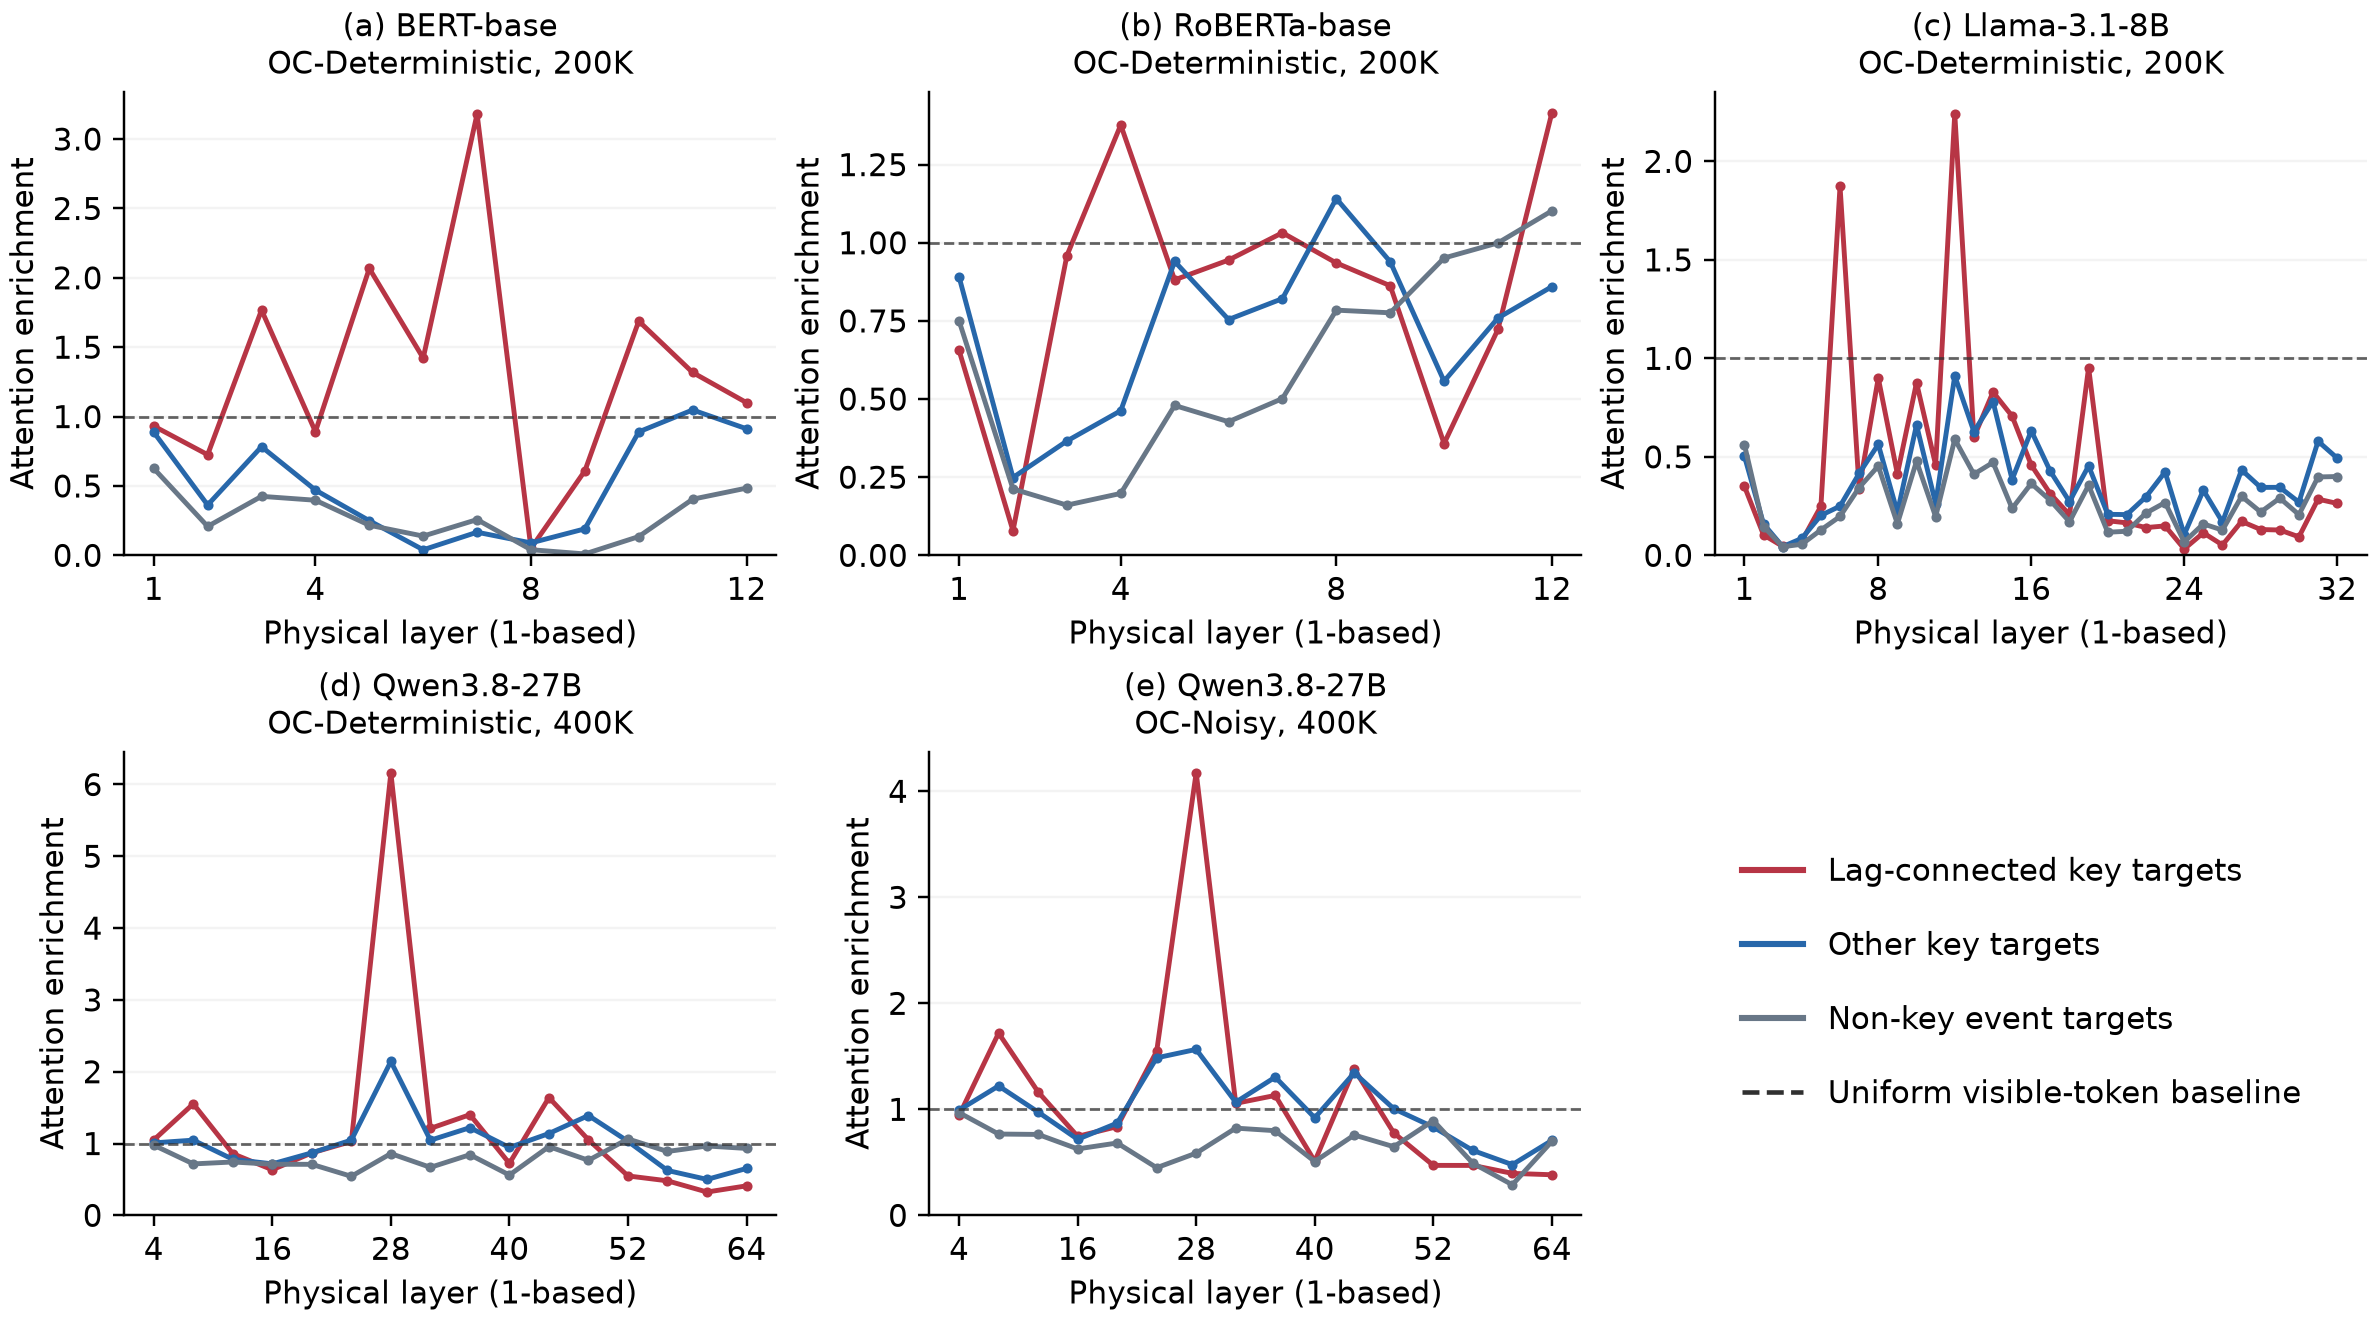
\includegraphics[width=\textwidth]{figures/attention_oc_profiles_20260925.png}
\caption{OC attention enrichment across physical layers for the five completed audits. Red: lag-connected key targets; blue: other key targets; gray: non-key event targets. Dashed lines indicate uniform attention over visible tokens. Curves average per-example enrichment over eligible examples and heads, using all sampled outcomes. Target categories have different eligibility sets. Layer numbering is one-based and panels use separate $y$-axis ranges. Qwen panels include standard attention blocks only. Localized lag enrichment is visible, but the profiles are descriptive and do not constitute a controlled architecture comparison or a causal attribution.}
\label{fig:attn_layer_summary}
\end{figure}

\paragraph{KIP: key-order sensitivity without a unique attention signature.}
We inspect 22 saved checkpoints on 1,000 fixed held-out examples per task: BERT-base and RoBERTa-base with full fine-tuning and LoRA on 4/6; Llama-3.2-1B with full fine-tuning on KIP-4/6; and Llama-3.1-8B LoRA,
Qwen2.5-14B QLoRA, and Qwen3.8-27B QLoRA on 4 at 4K, 40K, 120K, and 200K training examples. Their attention profiles show model-dependent key routing rather than a common preference for inversion pairs.  Figure~\ref{fig:attn_kip_summary} shows the four successful M4 checkpoints

\begin{figure}[t]
\centering
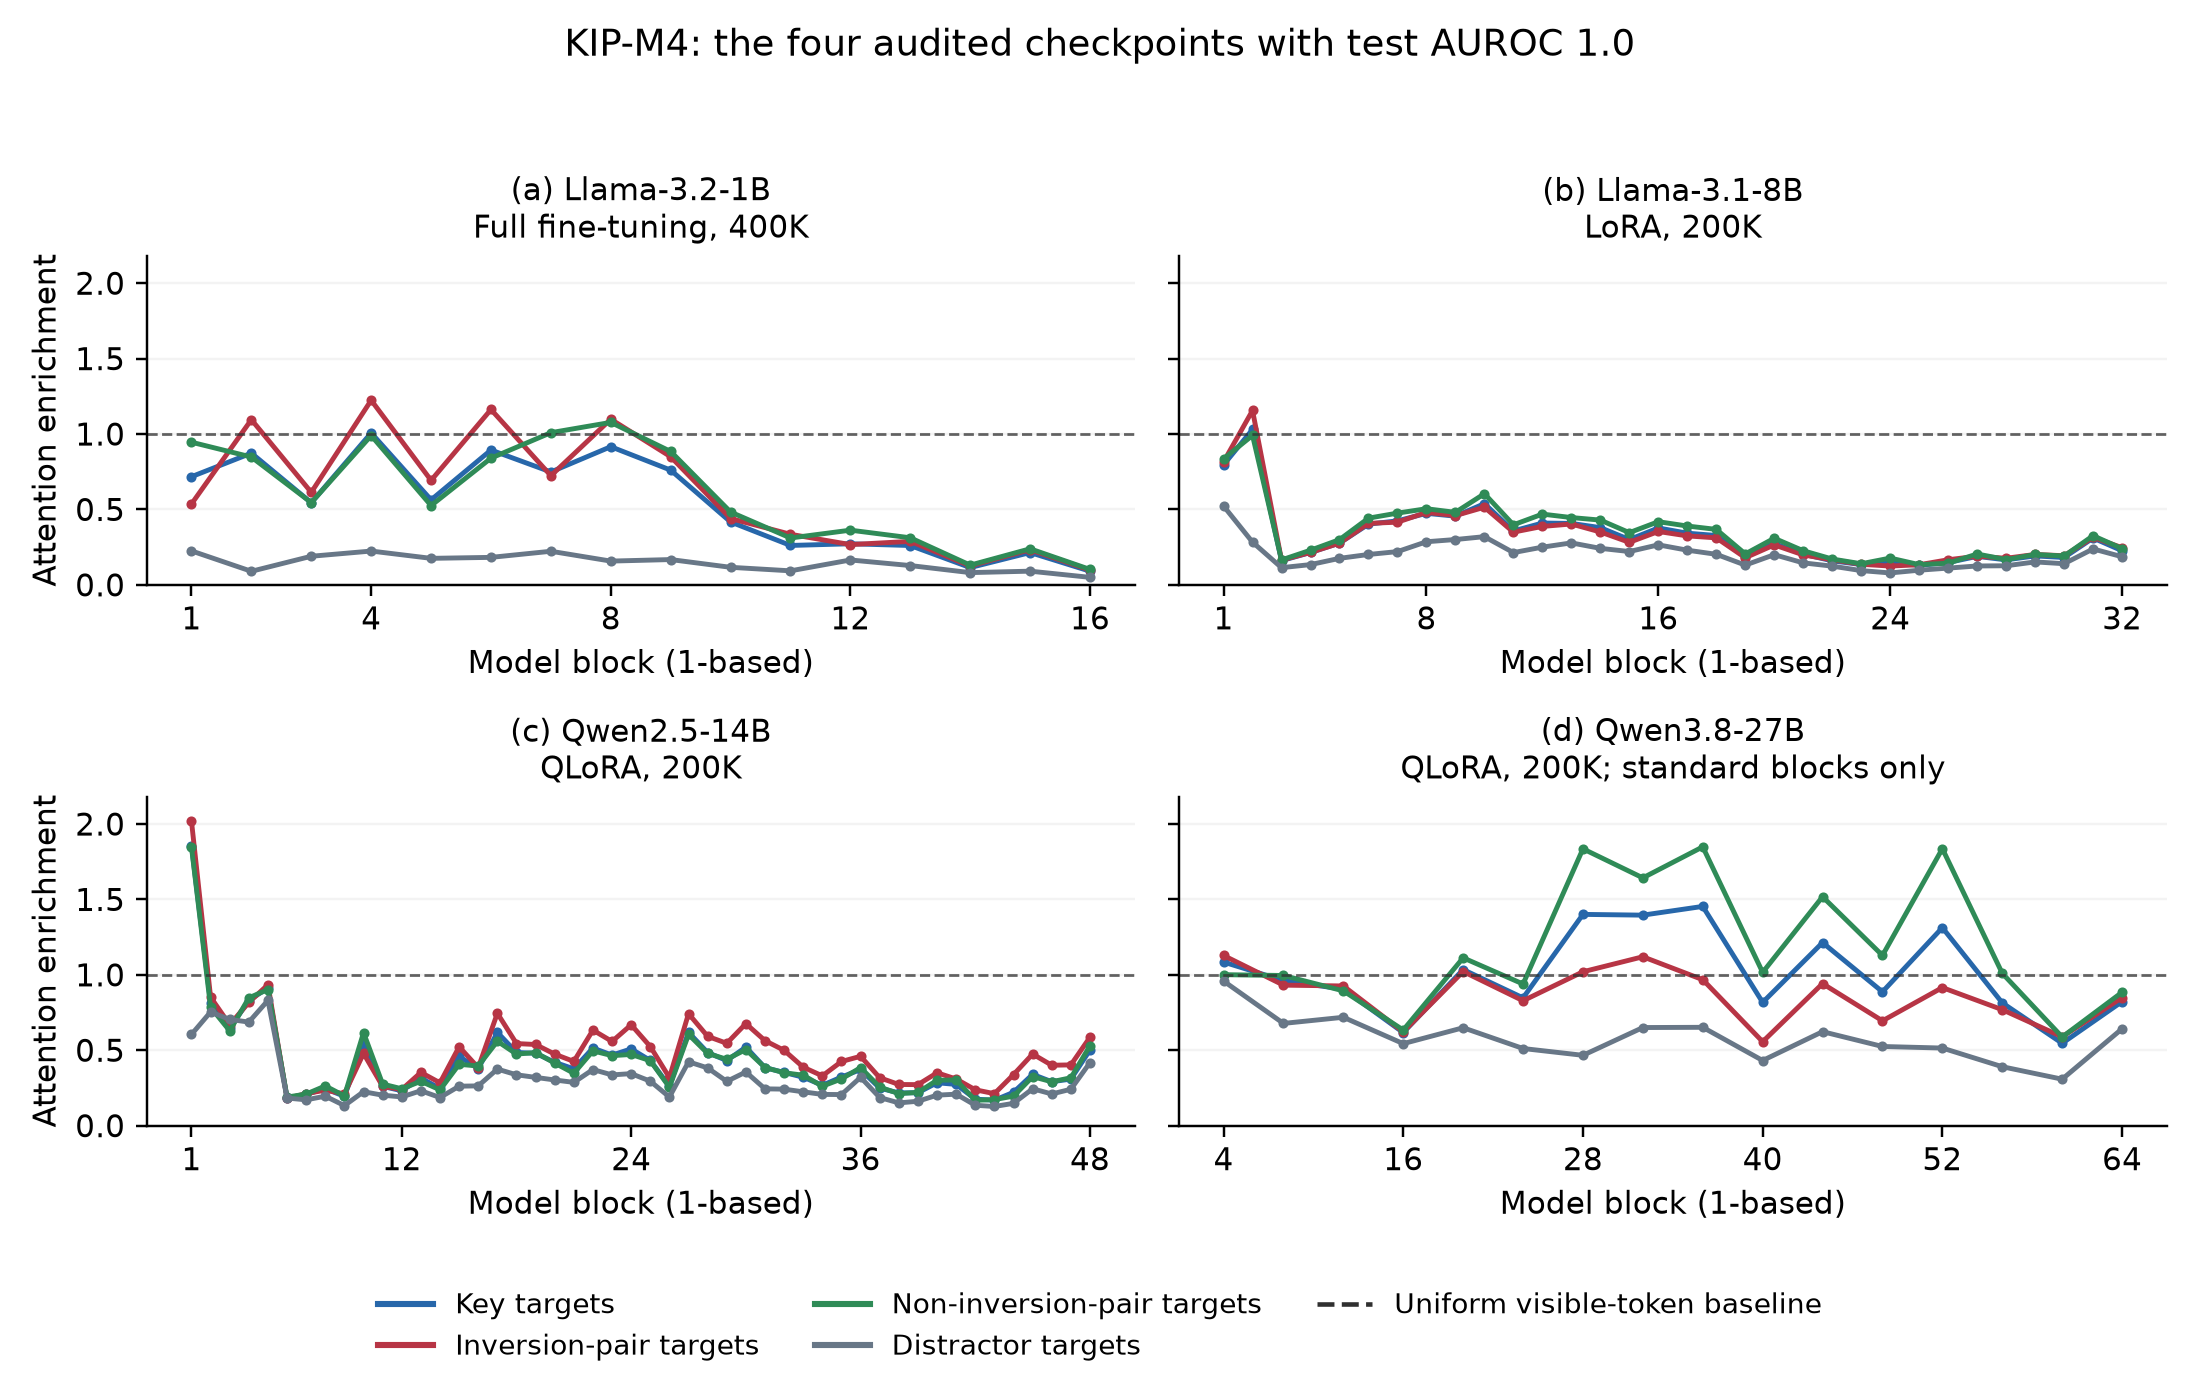
\includegraphics[width=\textwidth]{figures/attention_kip_m4_profiles_20260925.png}
\caption{Attention enrichment for the four audited KIP-M4 checkpoints with
test AUROC 1.0. Llama-3.2-1B uses full fine-tuning on 400K examples; the larger
decoders use LoRA or QLoRA on 200K. Blue: key targets excluding the source
event; red: inversion-pair targets; green: non-inversion-pair targets; gray:
distractors. Dashed lines denote uniform attention over all visible tokens,
including self and prompt/special tokens. Curves average per-example
mass-to-baseline ratios over eligible examples and then heads. Key and distractor
curves use all 1,000 sampled examples; inversion and non-inversion curves use
971 and 961 eligible examples, respectively. Categories overlap and conditional
averaging differs, so the curves are not additive. Model-block indices are
one-based. Only standard attention blocks are shown for Qwen3.8-27B; connecting
lines do not measure its intervening recurrent blocks. These selected-checkpoint
profiles describe model-dependent routing and do not identify an internal
parity algorithm or provide a controlled architecture comparison.}
\label{fig:attn_kip_summary}
\end{figure}

\paragraph{MIMIC-IV CKD attention analysis.}
For BERT-base, RoBERTa-base, Llama-3.1-8B, and Qwen3.8-27B, we compare separately trained ordered and shuffled models on the same 1,000 held-out patients, including 77 progressors. We inspect the classifier readout query (CLS for encoders, the last unmasked token for decoders); Qwen again contributes only its 16 standard attention blocks. We aggregate repeated CCS-code occurrences, average code masses over heads and audited layers, then normalize within each patient to sum to one over CCS codes, excluding prompt mass.
The mean paired overlap, defined as one minus total-variation distance between these code distributions, is 0.850 for BERT, 0.848 for RoBERTa, 0.703 for Llama, and 0.674 for Qwen. This describes shared allocation to clinical content, without identifying causal risk factors or proving order invariance. The comparison changes both model weights and input order. Moreover, encoders truncate at 512 tokens, affecting 191 BERT and 188 RoBERTa sampled patients, whereas both decoders retain full histories. Shuffling can change which events remain visible after truncation, precluding an equal-context architecture comparison. Figure~\ref{fig:attn_ckd_summary} visualizes the layer-wise allocation to diagnosis events and the dispersion of readout attention for both conditions.

\begin{figure}[t]
\centering
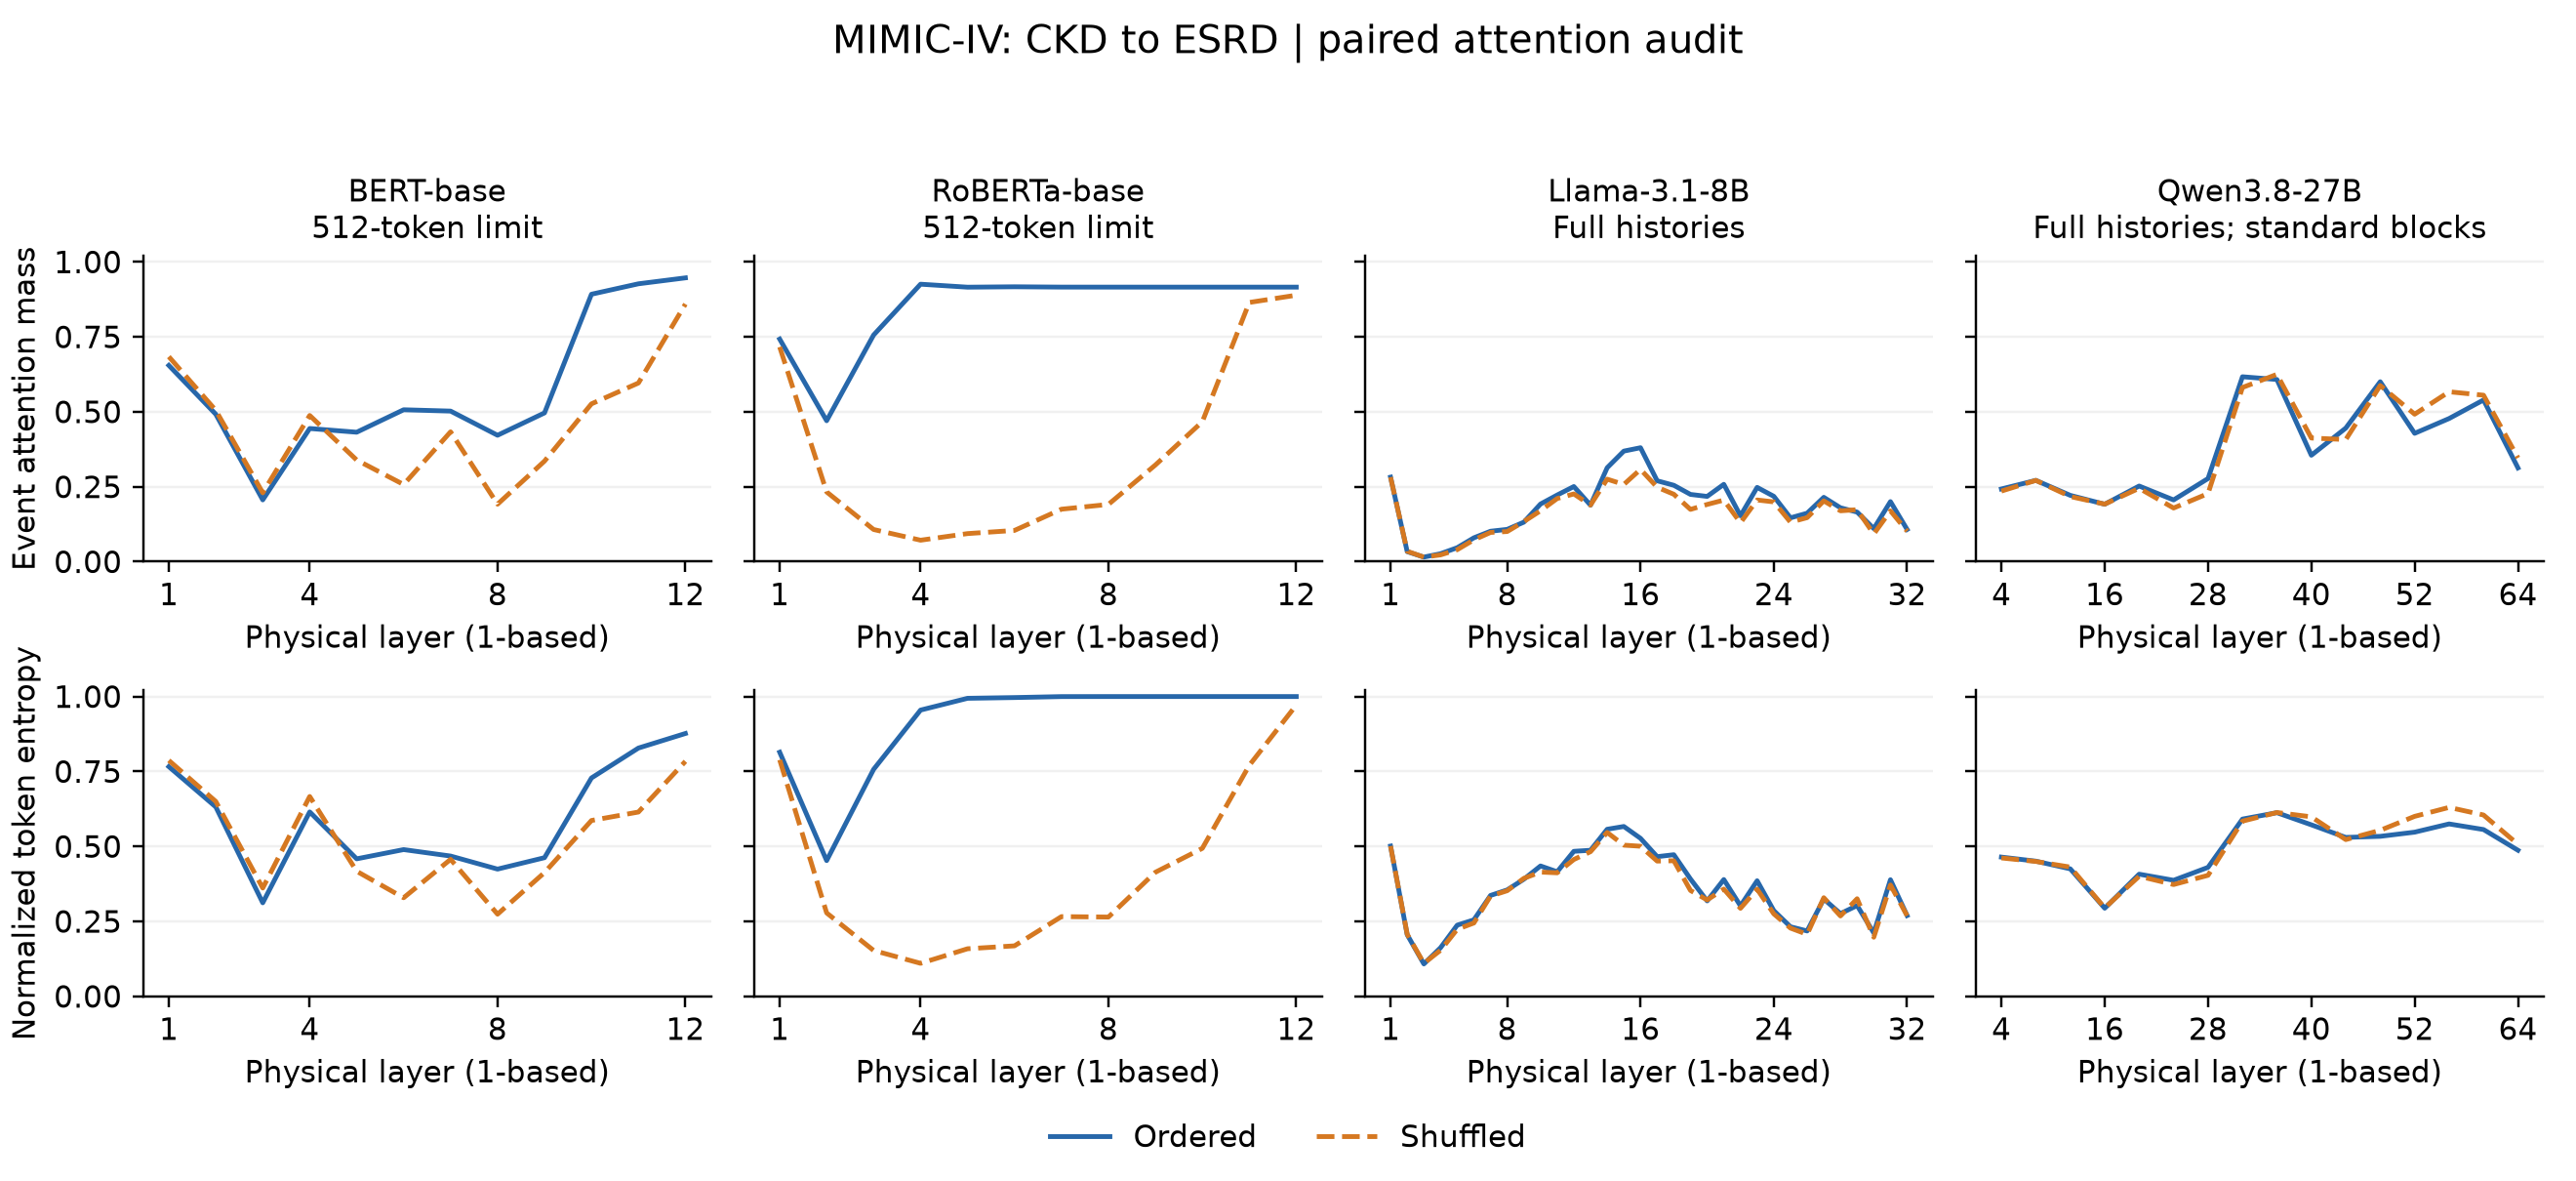
\includegraphics[width=\textwidth]{figures/attention_ckd_profiles_20260925.png}
\caption{MIMIC-IV CKD$\to$ESRD readout attention in separately trained ordered (solid blue) and shuffled (dashed orange) models on the same 1,000 held-out patients. Top: attention mass assigned to complete visible diagnosis events. Bottom: token-attention entropy normalized by the logarithm of the visible token count; higher values indicate more diffuse allocation. Both quantities are averaged over heads within each patient and then over patients at each physical layer. Encoders use the CLS query and a 512-token window; decoders use the last unmasked query and full histories. Qwen includes only its 16 standard attention blocks. Layers are numbered from one. Conditions differ in model weights and input order, and encoder truncation can change visible content. The profiles are descriptive, not a controlled comparison of architectures or causal effects
of shuffling.}
\label{fig:attn_ckd_summary}
\end{figure}

\end{document}
